% Title: Report LaTex File: Hardware Development
% Auther: DC Eksteen
% Student Number: 22623906
% Contact: 22623906@sun.ac.za
% Date: 2022/09/14
% Version: 2.0

\chapter{Hardware Development}
% Section overview: Hardware development.
\label{ch:hardware}
\section{Roller Design}
\label{sec:opspeed}

\subsection{Design Considerations}

Roller trainers require smooth and constant cycling for stable operation. The motion of the bicycle wheels are coupled to the roller drums by friction. Common drum sizes that are available on retail models range from \SI{80}{\milli\meter} to \SI{120}{\milli\meter} diameters and are constructed from either aluminium or PVC plastic. 

%For the development in this project, an operating range between \SI{10}{\kilo\meter\per\hour} and \SI{50}{\kilo\meter\per\hour} is considered according to PR~\ref{PR:speed}.

Figure~\ref{fig:Speed2} shows a comparison of the rotational speed expected for the designed operating conditions of different drum sizes. Figure~\ref{fig:Speed} shows the braking torque required to achieve \SI{400}{\watt} of braking power for each of the considered drum diameters.

\begin{figure}[H]
	\centering
	\begin{subfigure}[b]{.475\textwidth}
		\centering
		\includegraphics[width=\linewidth]{SpeedCalculations.jpg}
		\caption{Rotational Speeds of Roller Drums}
		\label{fig:Speed2}
	\end{subfigure}
	\hfill
	\begin{subfigure}[b]{.475\textwidth}
		\centering
		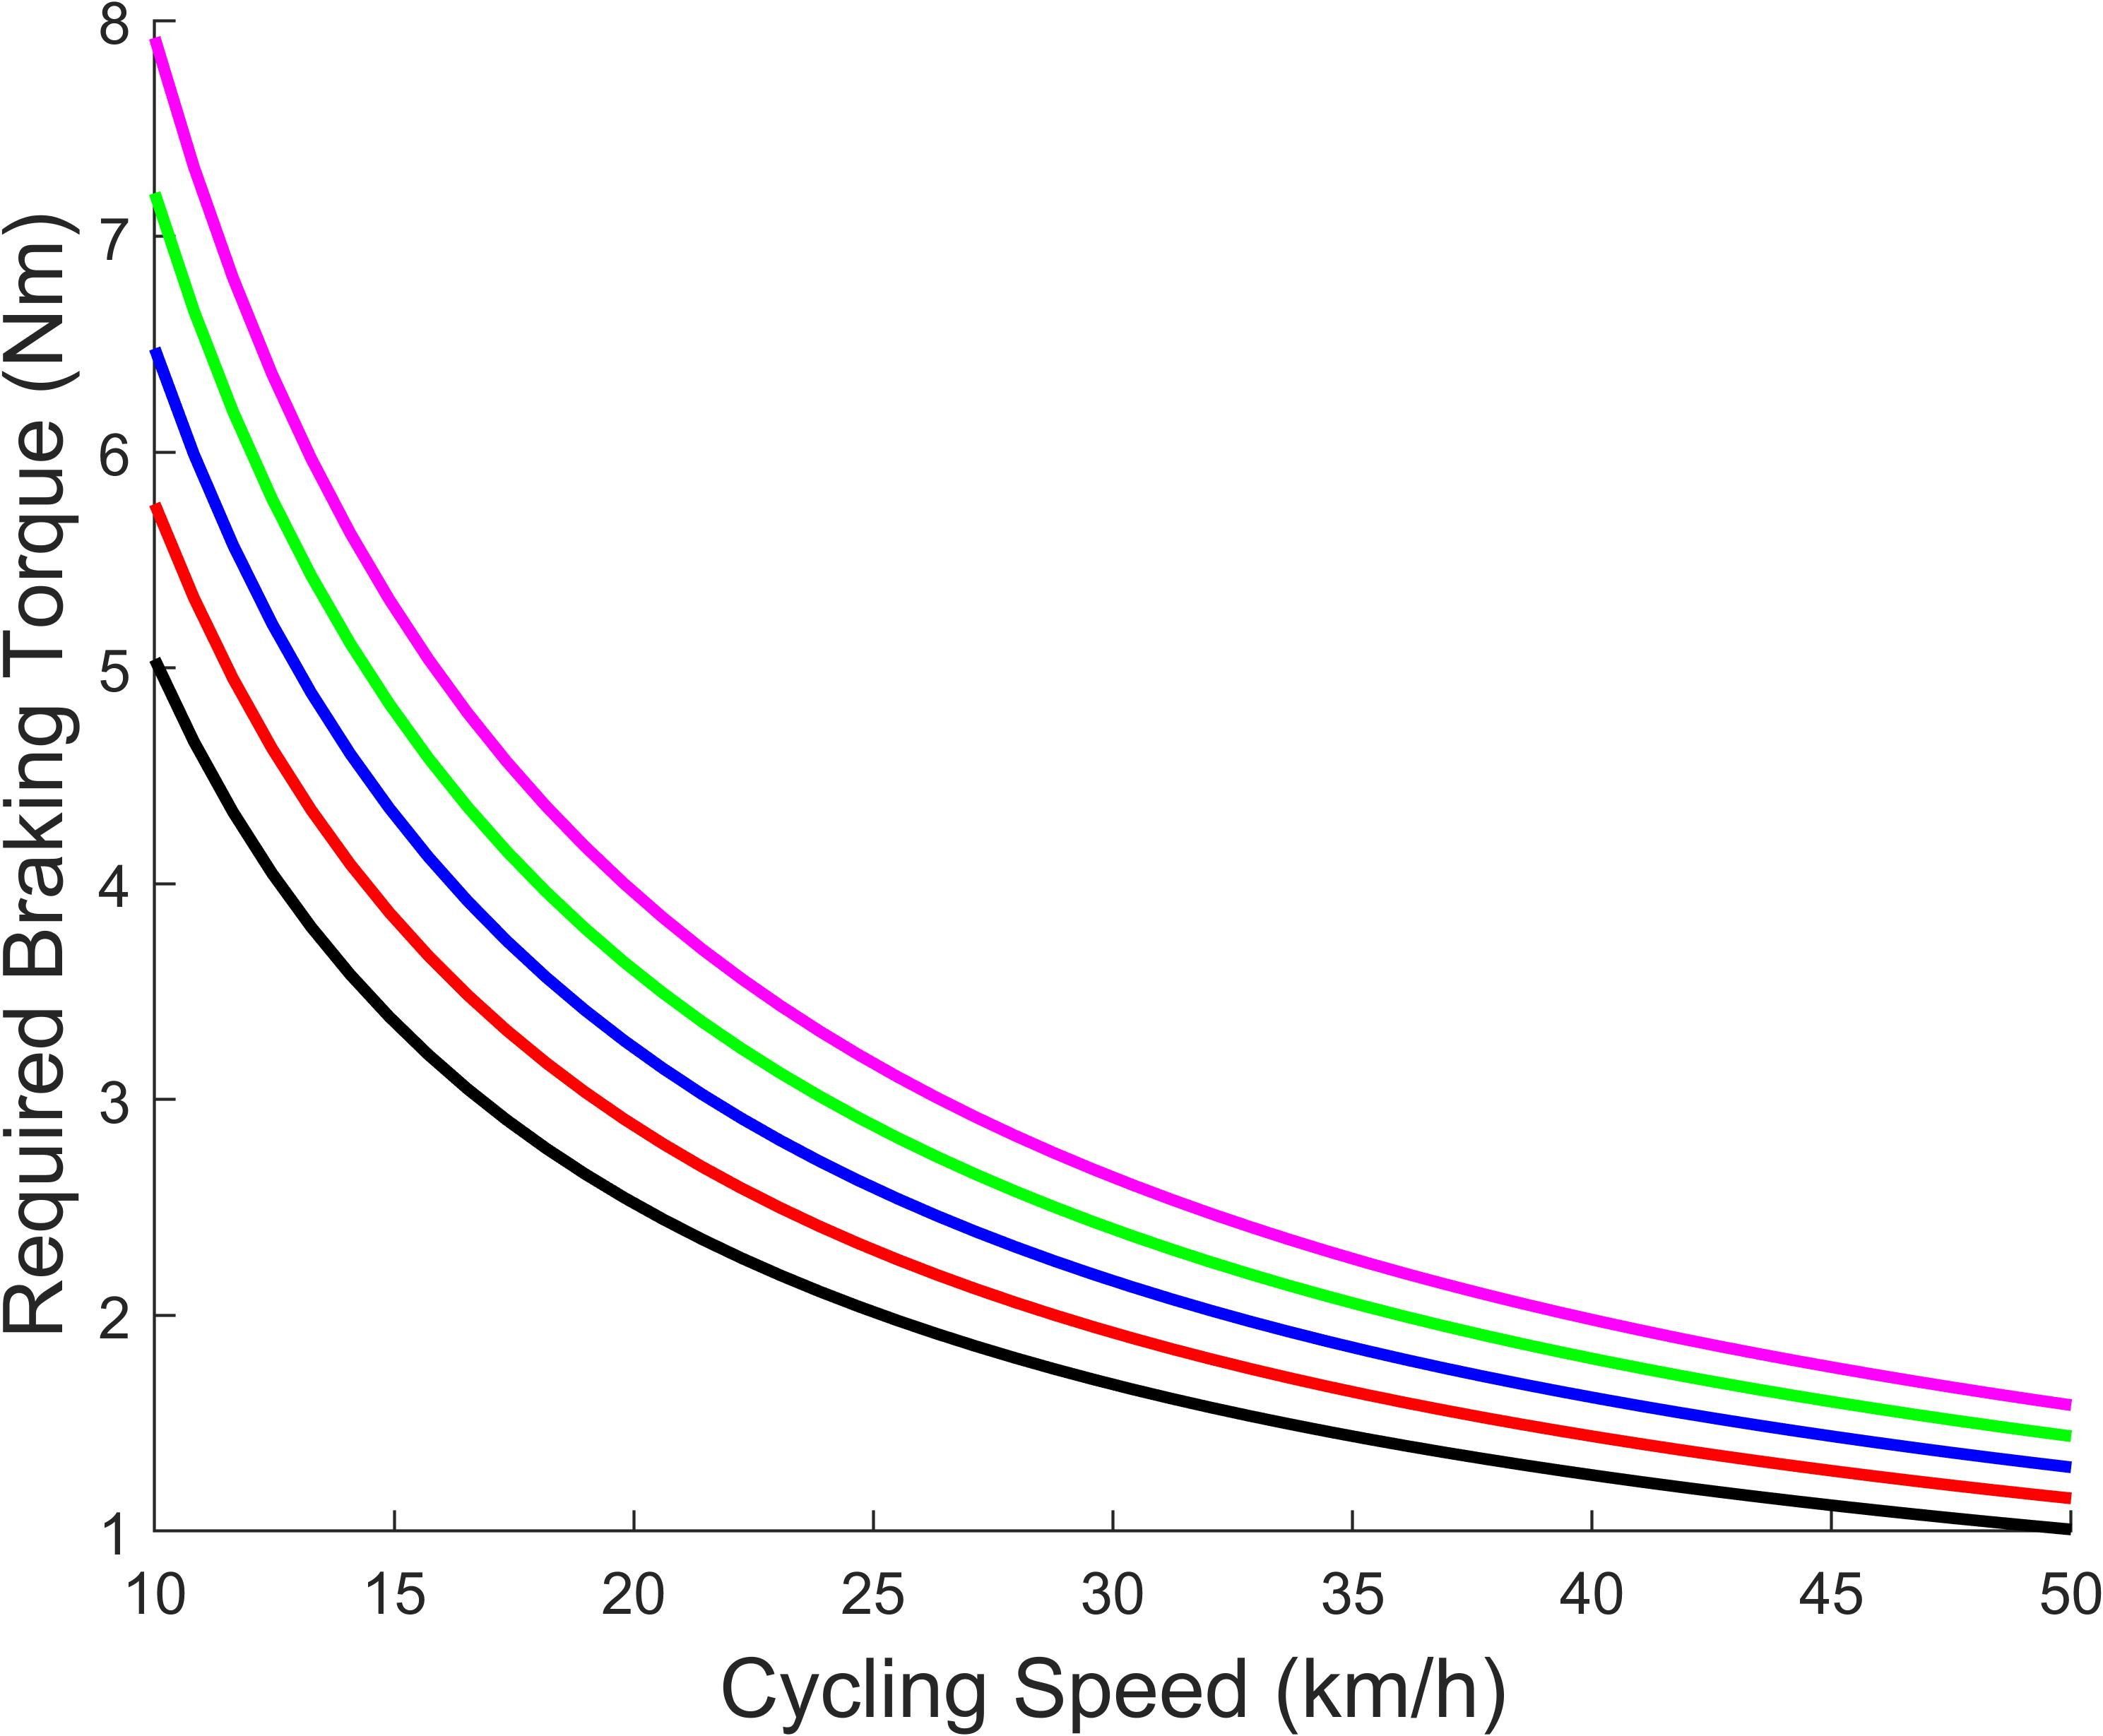
\includegraphics[width=\linewidth]{SpeedCalculations2.jpg}
		\caption{Requirement for \SI{400}{\watt} Braking Power}
		\label{fig:Speed}
	\end{subfigure}
	\begin{subfigure}{.475\textwidth}
		\centering
		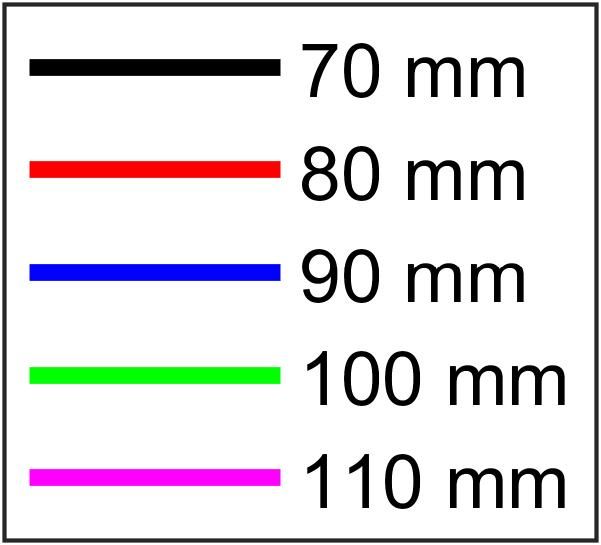
\includegraphics[width=0.3\linewidth]{SpeedLegend.jpg}
	\end{subfigure}
	\caption{Roller Drum Size Comparison}
	\label{fig:a}
\end{figure}

\vspace*{-0.5cm}	

Selection of the drum diameter to be used for the rollers was dominated by considerations for the eddy current brake discussed in Chapter~\ref{sec:Eddy}. Rollers with a smaller diameter drum will rotate at a higher angular velocity leading to higher braking torques achievable by the eddy current brake. Higher angular velocities also lead to a higher operating power floor as a higher rotational velocity leads to higher rolling resistance within the bearings.

\subsubsection{General Roller Design}

A diameter of \SI{90}{\milli\meter} was selected for the drum size as a good compromise between the advantages of higher and lower rotational velocities. The rollers were designed to consist of class-12 \acf{upvc} pipes as this is a much more affordable option than aluminium. Class-12 \ac{upvc} pipes are typically used in high pressure applications and are thus designed to handle higher loads than normal store-bought PVC pipes. 

The roller shafts are constructed out of EN-8 engineering steel. Figure~\ref{fig:rollerGen} shows the general design of the rollers that will be used for the trainer.

\begin{figure}[H]
	\centering
	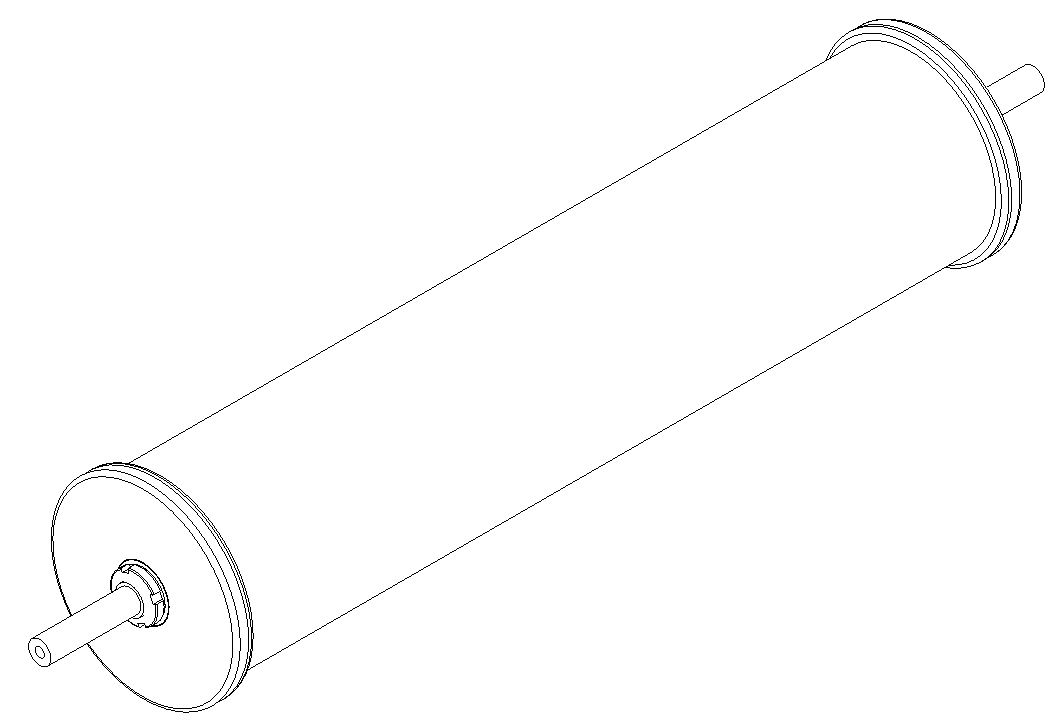
\includegraphics[width=0.4\linewidth]{rollerCad.jpg}
	\caption{Designed Roller Assembly}
	\label{fig:rollerGen}
\end{figure}

Three rollers were needed for the trainer and two types of rollers were designed for this project. The two front rollers would serve as idle rollers and the rear roller will be used to apply the braking force. 

\subsubsection{Bearing Selection}

690-2RS deep groove ball bearings with rubber shields on both sides were selected for the rollers. The bearings have a rated operating temperature range between \SI{-80}{\degreeCelsius} and \SI{300}{\degreeCelsius} with a rated maximum operating speed of 36,000 \ac{rpm}. The rubber shields serve to keep contaminants out of the bearings, leading to a longer usable operational life. 

\subsection{Idle Roller Design}

Figure~\ref{fig:idlecut} is a cross sectional representation of the designed idle roller where the final result seen in Figure~\ref{fig:rollerBuild} shows the addition of a segmented sticker used by the rotary encoder tachometer measuring the roller speed.

The idle roller drums are mounted on two pairs of bearings at each end cap. This allows for even distribution of radial loads and will lead to a higher expected operational life. 

\begin{figure}[H]
	\centering
	\begin{subfigure}{.5\textwidth}
		\centering
		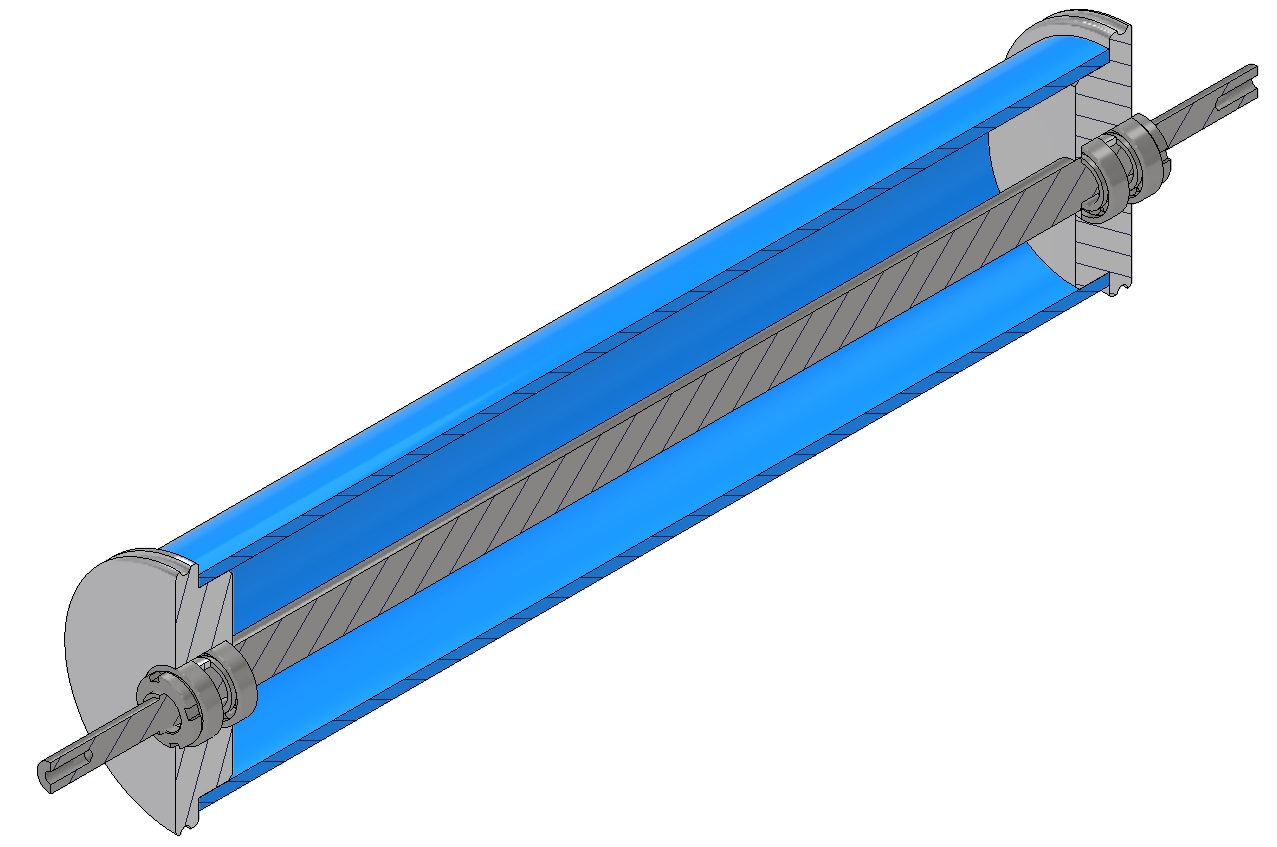
\includegraphics[width=\linewidth]{IdleRollerCut.jpg}
		\caption{Design Cross Section}
		\label{fig:idlecut}
	\end{subfigure}%
	\begin{subfigure}{.5\textwidth}
		\centering
		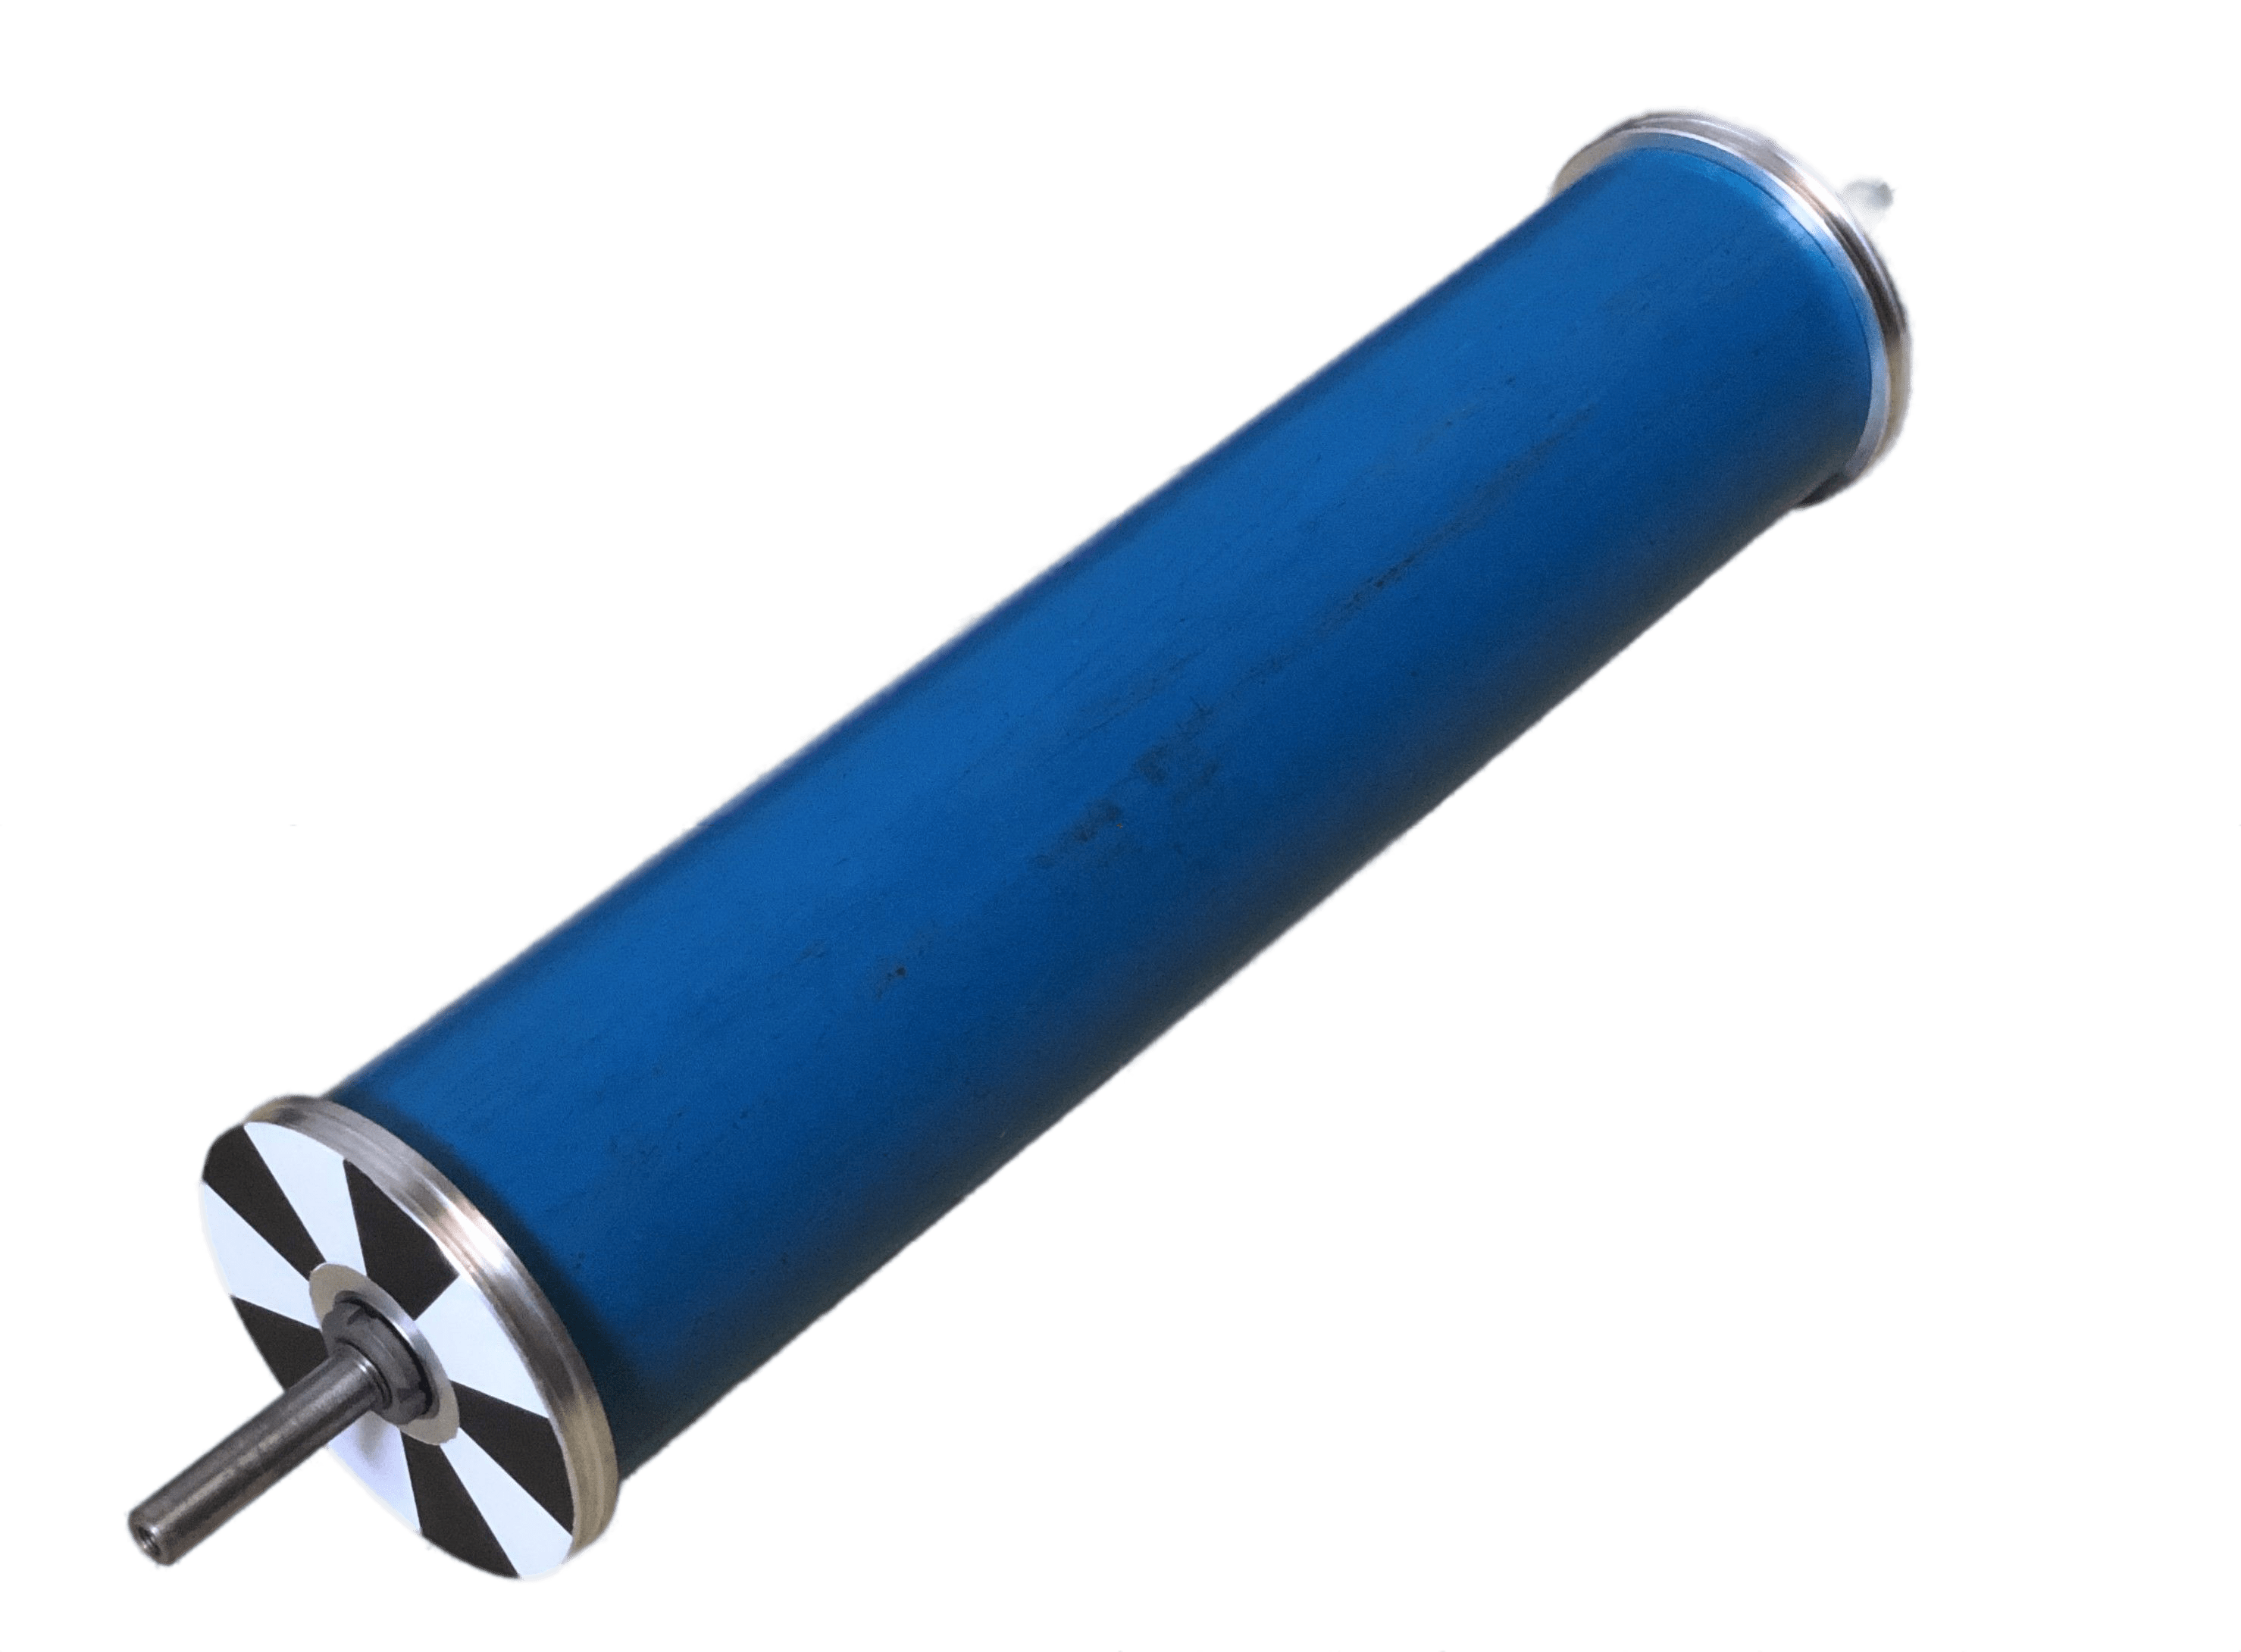
\includegraphics[width=\linewidth]{rollerBuilt.jpg}
		\caption{Final Built Roller}
		\label{fig:rollerBuild}
	\end{subfigure}
	\caption{Idle Roller}
	\label{fig:rollerdets}
\end{figure}

\vspace*{-0.9cm}

The roller assembly is held together with a lock nut on each side allowing for easy disassembly for maintenance or replacement of parts in the future. The idle rollers are attached to the trainer frame using M8 bolts threaded into each end of the shaft.

\subsection{Power Roller Design}

Figure~\ref{fig:rollerCAD} shows a cross sectional sketch of the designed power roller. The eddy current brake was implemented on the one end of the power roller, allowing for variable resistance to be applied to the bicycle during a training session.

\begin{figure}[H]
	\centering
	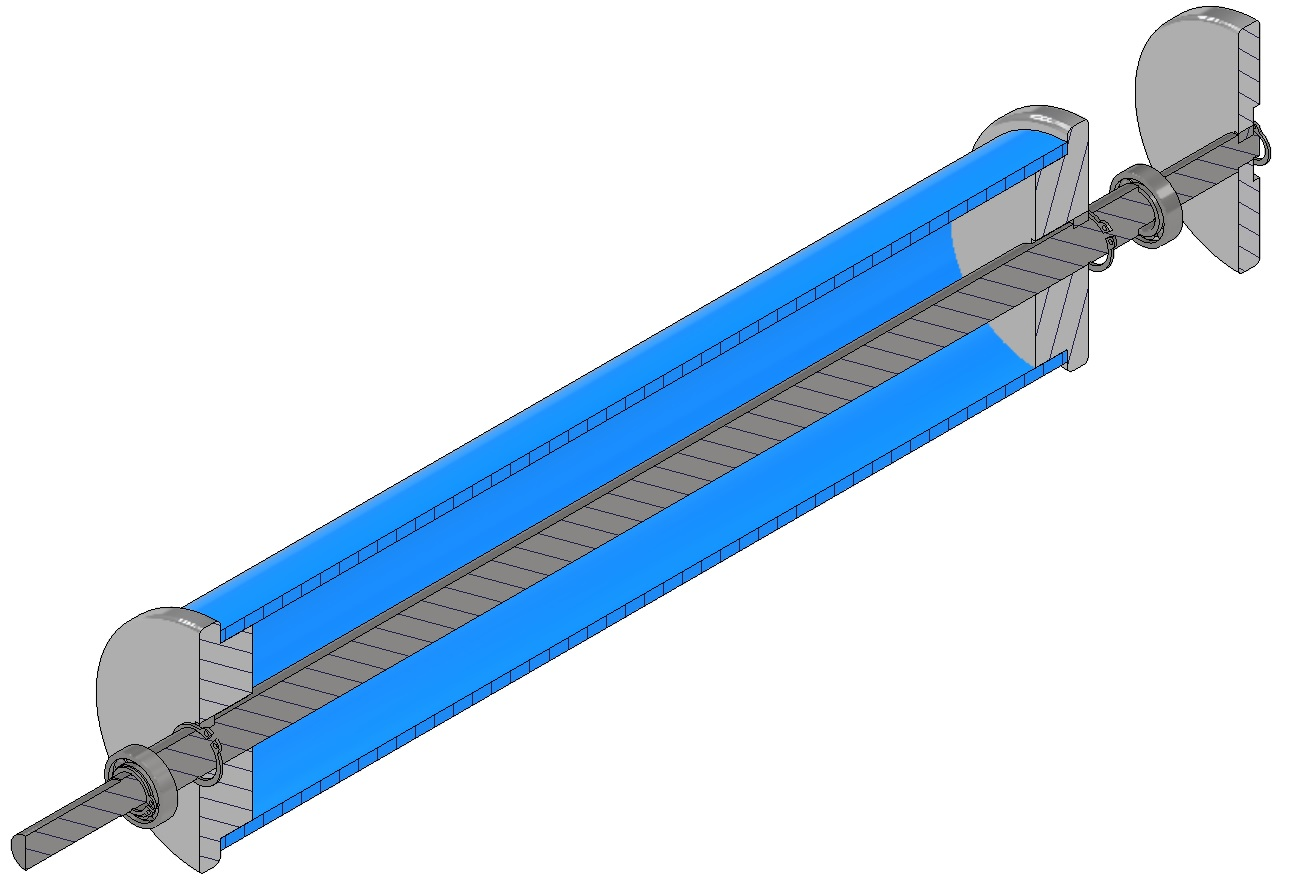
\includegraphics[width=0.62\linewidth]{PowerRollerCut.jpg}
	\caption{Power Roller Cross Section}
	\label{fig:rollerCAD}
\end{figure}

The power roller drum is rigidly attached to the roller shaft by a key at each of its aluminium end caps. An aluminium braking disk is also attached to one end of the roller shaft and held in position by a circlip. The side opposite the braking disk is designed to be exposed to allow for testing of the trainer and braking unit after assembly is completed.

%%%%%%%%%%%%%%%%%%%%%%%%%%%%%%%%%%%%%%%%%%%%%%%%%%%%%%%%%%%%%%%%%%%%%%%%%%%%%%%%%%%%%%%%%%%%%%%%%%%%%%%%%%%%%%%%%
%%%%%%%%%%%%%%%%%%%%%%%%%%%%%%%%%%%%%%%%%%%%%%%%%%%%%%%%%%%%%%%%%%%%%%%%%%%%%%%%%%%%%%%%%%%%%%%%%%%%%%%%%%%%%%%%%
%%%%%%%%%%%%%%%%%%%%%%%%%%%%%%%%%%%%%%%%%%%%%%%%%%%%%%%%%%%%%%%%%%%%%%%%%%%%%%%%%%%%%%%%%%%%%%%%%%%%%%%%%%%%%%%%%

\section{Eddy Current Brake Design}
\label{sec:Eddy}

%\subsubsection{Braking Torque Requirements}

Figure~\ref{fig:torqueCalc} shows the braking torque requirements for achieving different braking power levels when \SI{90}{\milli\meter} roller drums are used. Since the brake disk is rotating at the same speed as the roller, the working speed for the eddy current brake will range between 590 \ac{rpm} and 2950 \ac{rpm}.

\begin{figure}[H]
	\begin{center}
		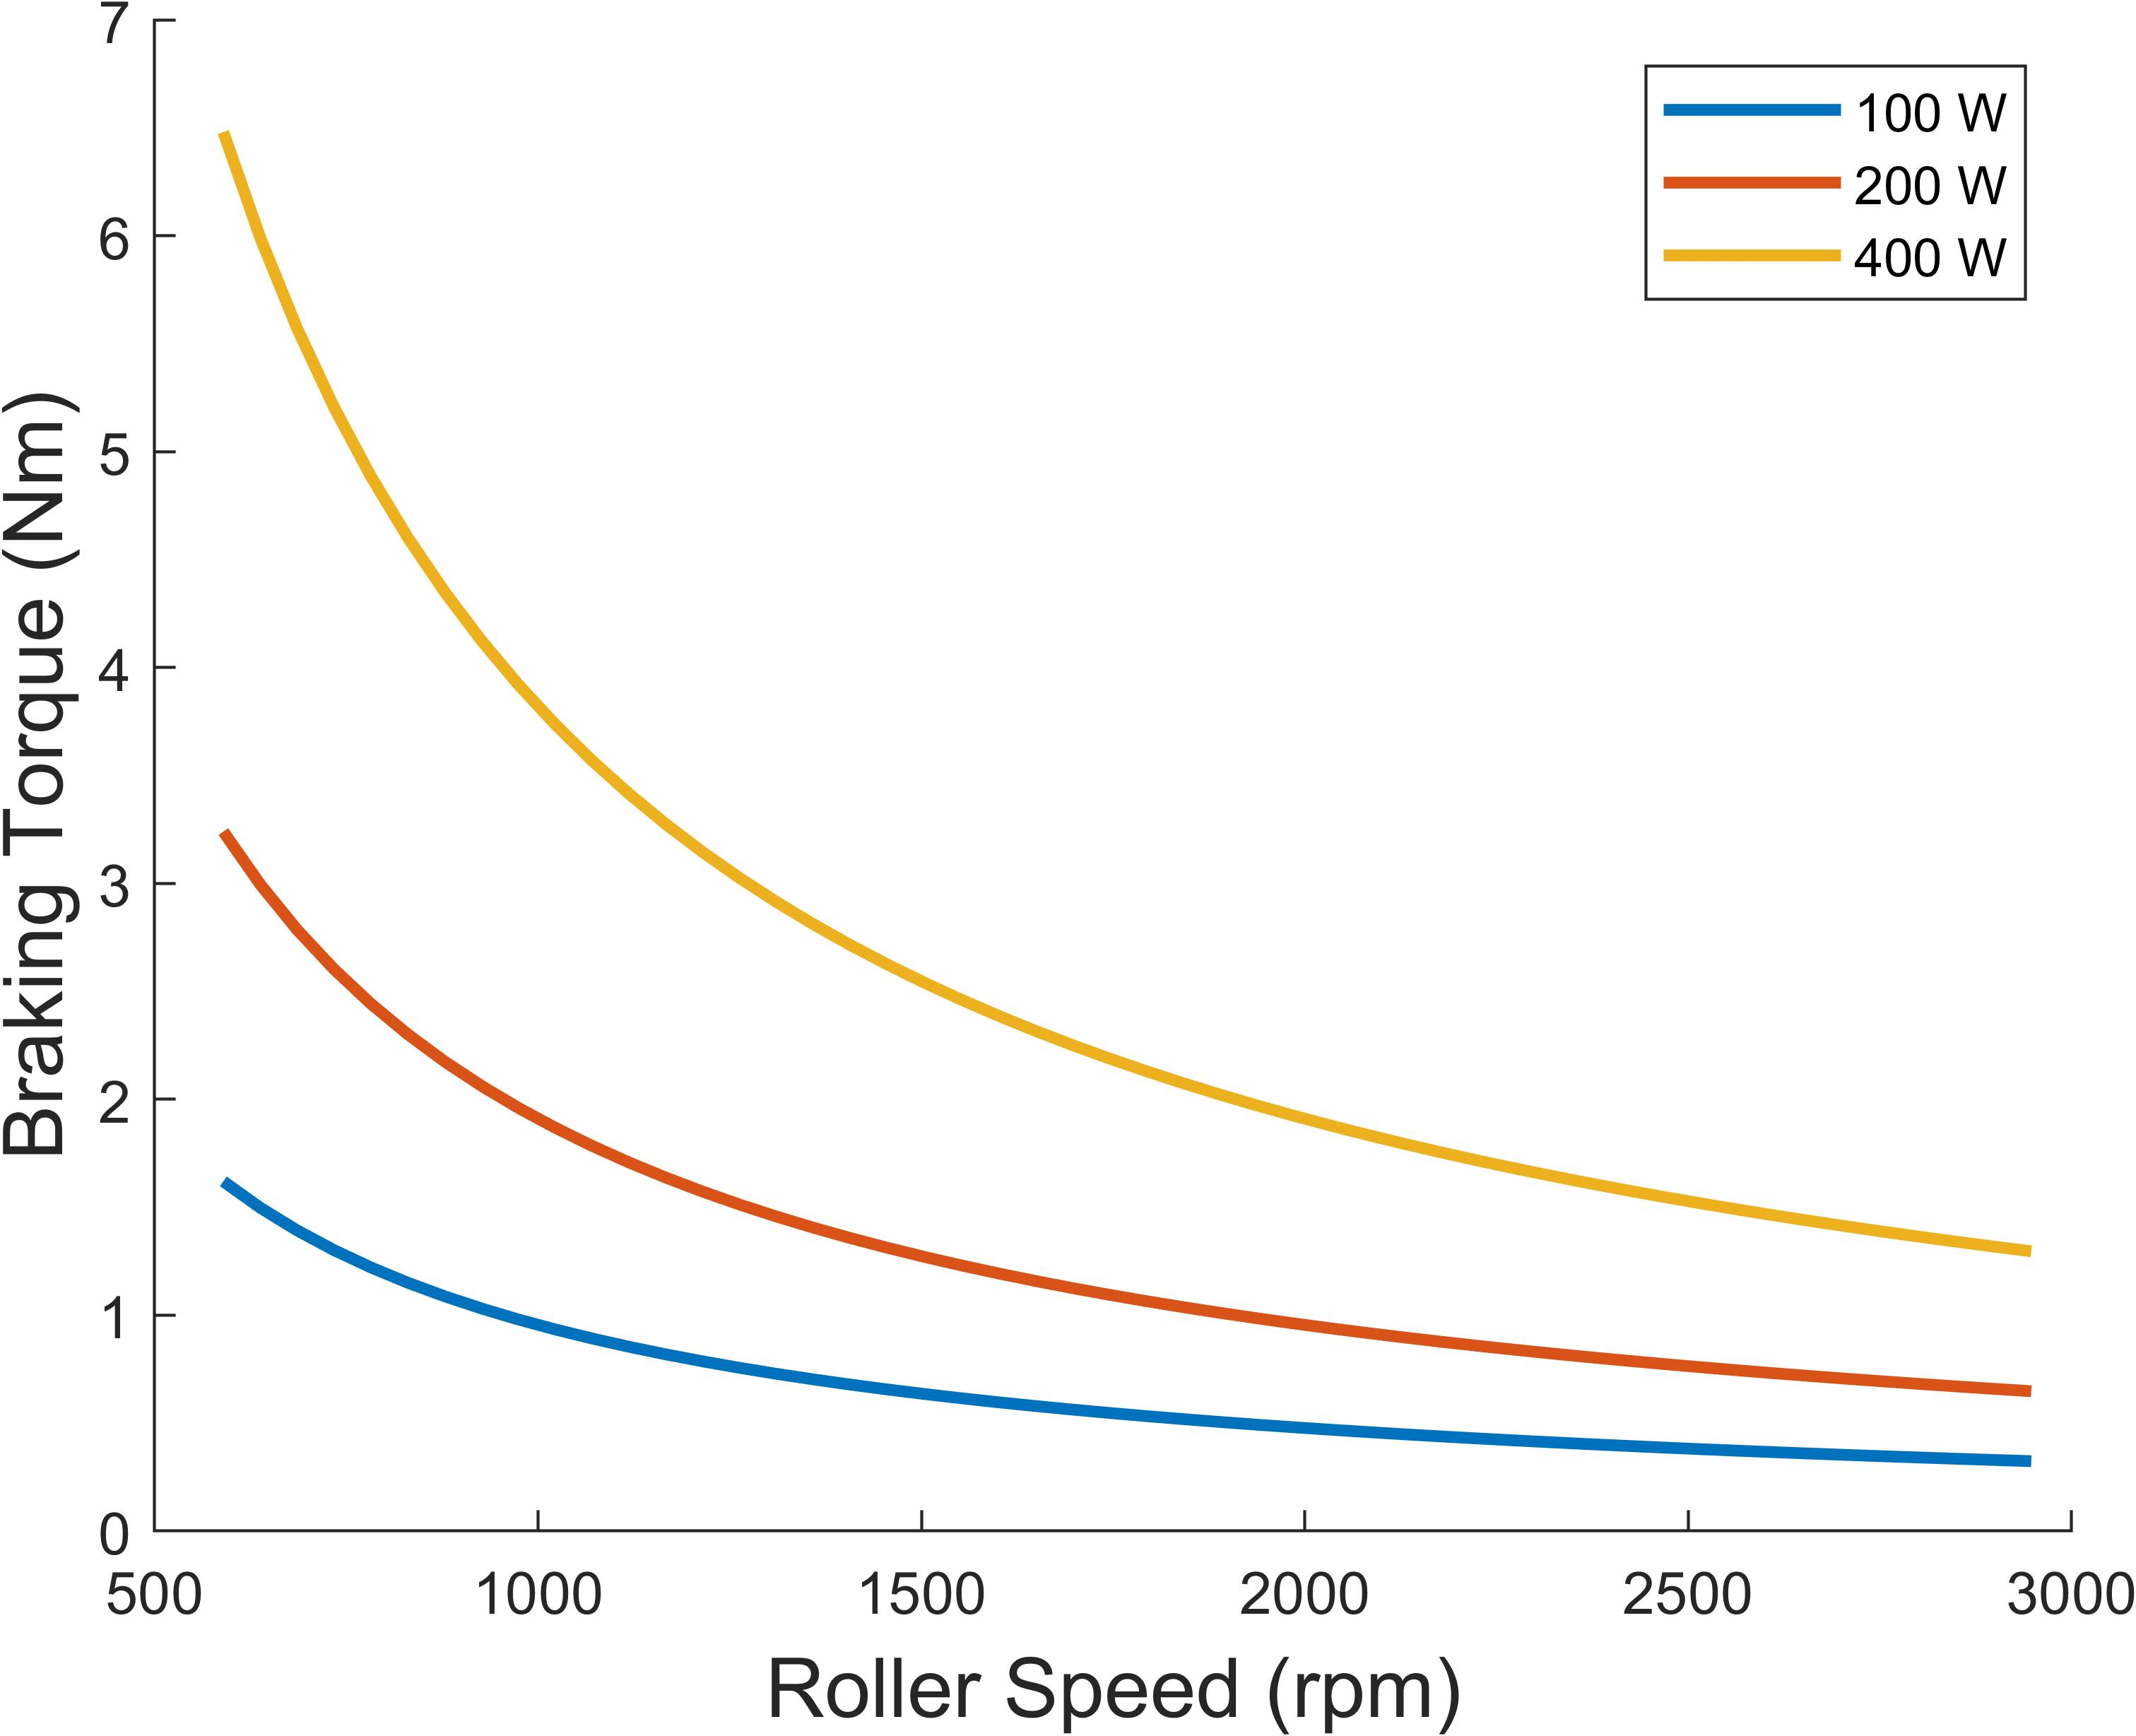
\includegraphics[width=0.6\textwidth]{TorqueCalculations.jpg}
		\caption{Torque Requirement Curve}
		\label{fig:torqueCalc}
	\end{center}
\end{figure}

\vspace{-0.9cm}

\subsection{Iron Backing}

The eddy current brake implemented in this project consists of two permanent magnet arrays with a conductive braking disk between them. The permanent magnets have an iron backing that serves to contain and concentrate the magnetic field lines between the magnets. This effect is demonstrated in Figure~\ref{fig:magconf}, where Figure~\ref{fig:magiron} shows an array with iron backing indicated by more concentrated magnetic field lines than in Figure~\ref{fig:magnoiron} showing an array with no iron backing. 

\begin{figure}[H]
	\centering
	\begin{subfigure}{.5\textwidth}
		\centering
		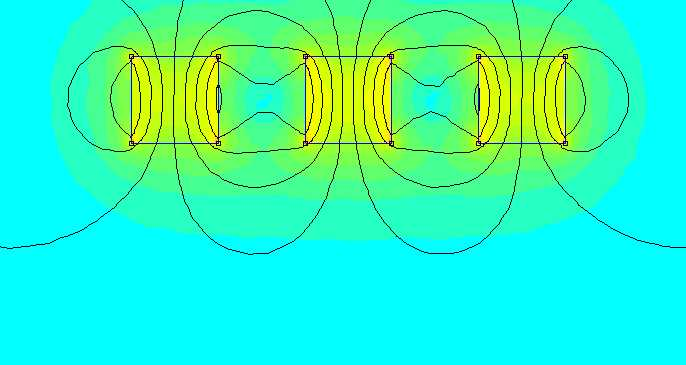
\includegraphics[width=0.8\linewidth]{MagnetsNoIron.jpg}
		\caption{Without Iron Backing}
		\label{fig:magnoiron}
	\end{subfigure}%
	\begin{subfigure}{.5\textwidth}
		\centering
		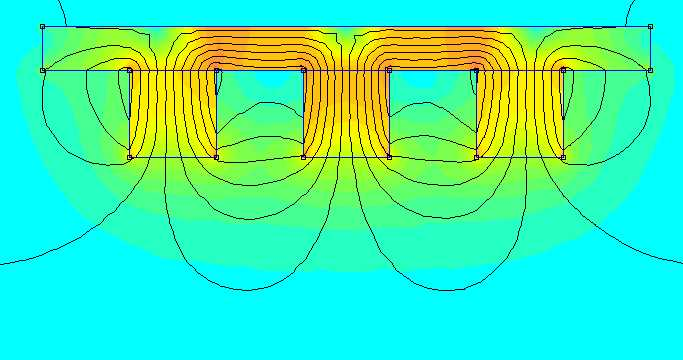
\includegraphics[width=0.8\linewidth]{MagnetsIron.jpg}
		\caption{With Iron Backing}
		\label{fig:magiron}
	\end{subfigure}
	\caption{Alternating Polarity Permanent Magnet Array}
	\label{fig:magconf}
	\citep{Parsons:2018}
\end{figure}

\vspace*{-0.5cm}

\subsection{Braking Torque Control}

Figure~\ref{fig:Electro} demonstrates that the total magnetic flux density between two permanent magnets can be found by super-imposing the magnetic flux density of each magnet at a given point. If magnets face each other with opposing poles, the magnetic flux density will add, and if the magnets face each other with the same pole, the magnetic density will cancel.

\begin{figure}[H]
	\centering
	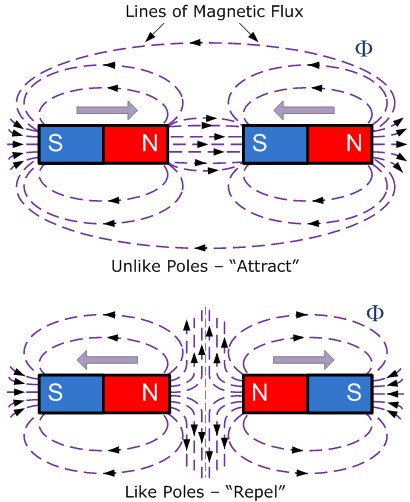
\includegraphics[width=0.3\textwidth]{electromagnetism.jpg}
	\caption{Attracting and Repelling Magnetic Flux Lines}
	\label{fig:Electro}
	\citep[2022]{electronics:2022}
\end{figure}

This phenomenon is what causes attraction and repulsion between magnetic poles. In the case of the eddy current brake designed for this project, the permanent magnets array configuration is shown in Figure~\ref{fig:MagsA}. The two arrays are then placed opposing each other with the aluminium brake disk between them as shown in Figure~\ref{fig:maxMags} and Figure~\ref{fig:minMags}.

\begin{figure}[H]
	\centering
		\begin{subfigure}{.3\textwidth}
		\centering
		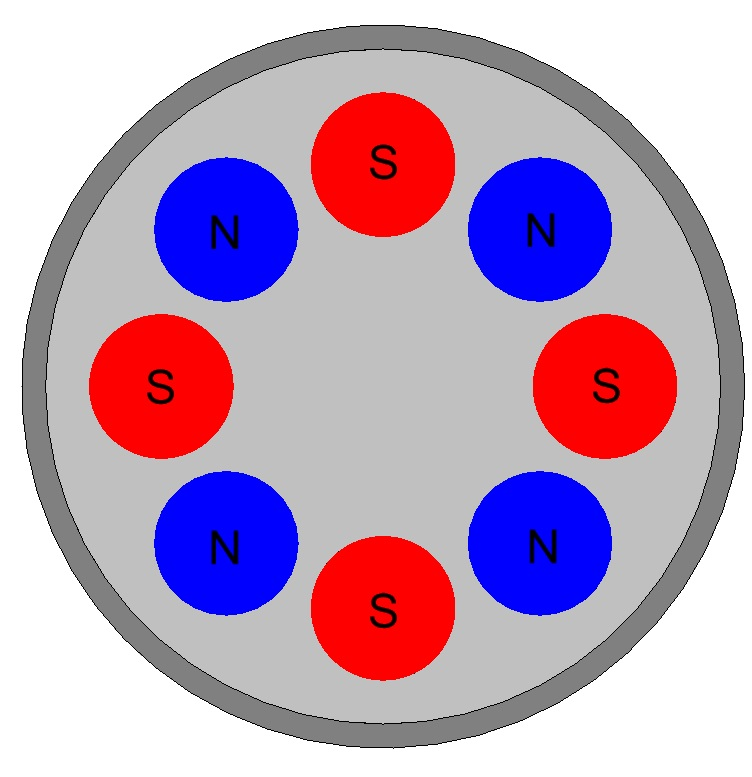
\includegraphics[height=\linewidth]{BrakeArrayBig.jpg}
		\caption{Array Configuration}
		\label{fig:MagsA}
	\end{subfigure}%
	\hfill
	\begin{subfigure}{.3\textwidth}
		\centering
		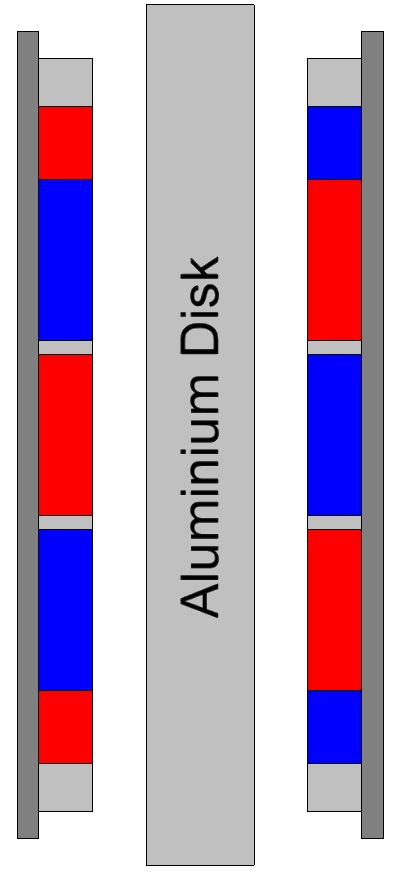
\includegraphics[height=\linewidth]{BrakeArrayMax.jpg}
		\caption{Maximum Braking}
		\label{fig:maxMags}
	\end{subfigure}%
	\hfill
	\begin{subfigure}{.3\textwidth}
		\centering
		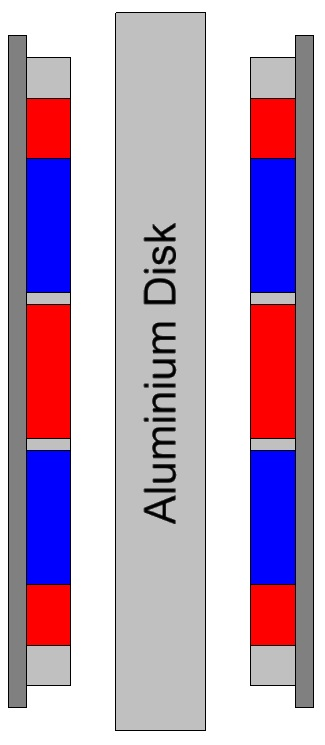
\includegraphics[height=\linewidth]{BrakeArrayMin.jpg}
		\caption{Minimum Braking}
		\label{fig:minMags}
	\end{subfigure}
	\caption{Braking Torque Control Design}
	\label{fig:magarrays}
\end{figure}

\vspace*{-0.5cm}

The aluminium disk will experience maximum braking torque when the arrays are orientated with opposite poles directly facing each other as shown in Figure~\ref{fig:maxMags}. On the other hand, the braking torque will be at it's minimum when the magnet arrays are orientated such that similar poles are directly opposing each other, as is shown in Figure~\ref{fig:minMags}.

\subsection{Parameter Selection}

Using the mathematical model demonstrated in Chapter~\ref{sec:ecb}, the final parameters for the eddy current brake were determined through many iterations. Rare earth magnets were used as they provide the highest magnetic flux density of any permanent magnets.

For the final brake design, 18 N38 Neodymium disc magnets with a diameter ($2r$) of \SI{15}{\milli\meter}, thickness ($t$) of \SI{5}{\milli\meter} and Bremenance field ($B_r$) of \SI{1.3}{\tesla} were used. Figure~\ref{fig:magN} is an example of the selected disk magnets. 

Equation~\ref{eq:B} was used to determine the magnetic field density ($B$) passing through the aluminium disk. Figure~\ref{fig:B0} indicates the direction ($z$) where the field density is calculated in Equation~\ref{eq:B}.

\begin{equation}
	\acs{B} = \frac{\acs{Br}}{2} (\frac{t+ z}{\sqrt{r^2 + {t + z}^2}} - \frac{z}{r^2 + z^2})
	\label{eq:B}
\end{equation}

\begin{figure}[H]
	\centering
	\begin{subfigure}{.4\textwidth}
		\centering
		\includegraphics[height=0.6\linewidth]{magnetD.jpg}
		\caption{Neodymium Disk Magnet}
		\label{fig:magN}
	\end{subfigure}%
\hfill
	\begin{subfigure}{.4\textwidth}
		\centering
		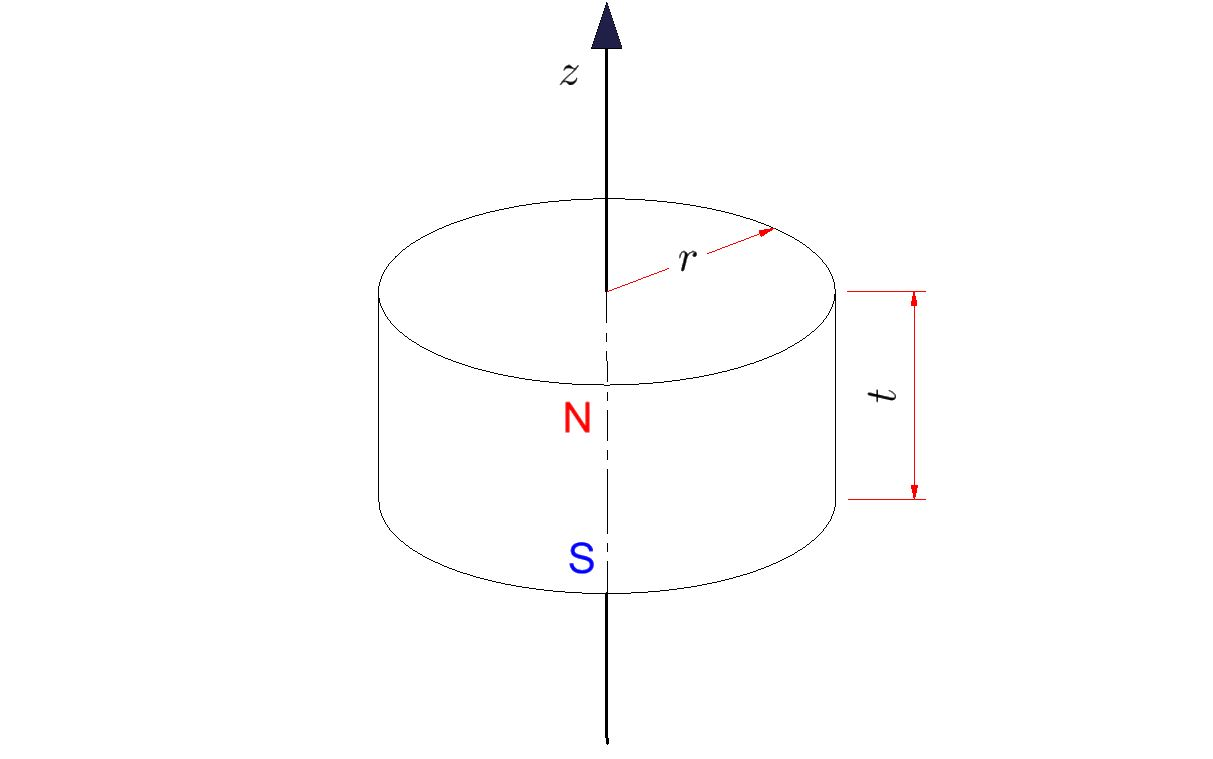
\includegraphics[height=0.6\linewidth]{magnetBr.jpg}
		\caption{\ac{B} Field Calculation}
		\label{fig:B0}
	\end{subfigure}
	\caption{Disk Magnet}
	\citep[Addapted from][]{Supermagnete:2010}
	\label{fig:magnets}
\end{figure}

\vspace*{-0.5cm}

The magnets are arranged in an alternating pole array as shown in Figure~\ref{fig:magarr} with \SI{3}{\milli\meter} thick EN-8 steel used as backing iron. The aluminium brake disk has a thickness of \SI{10}{\milli\meter} and a diameter of \SI{90}{\milli\meter}. The air gap between the brake disk and each magnet array is \SI{3}{\milli\meter}. Figure~\ref{fig:brakefin} shows the configuration of the final built eddy current brake.

\begin{figure}[H]
	\centering
	\begin{subfigure}{.4\textwidth}
		\centering
		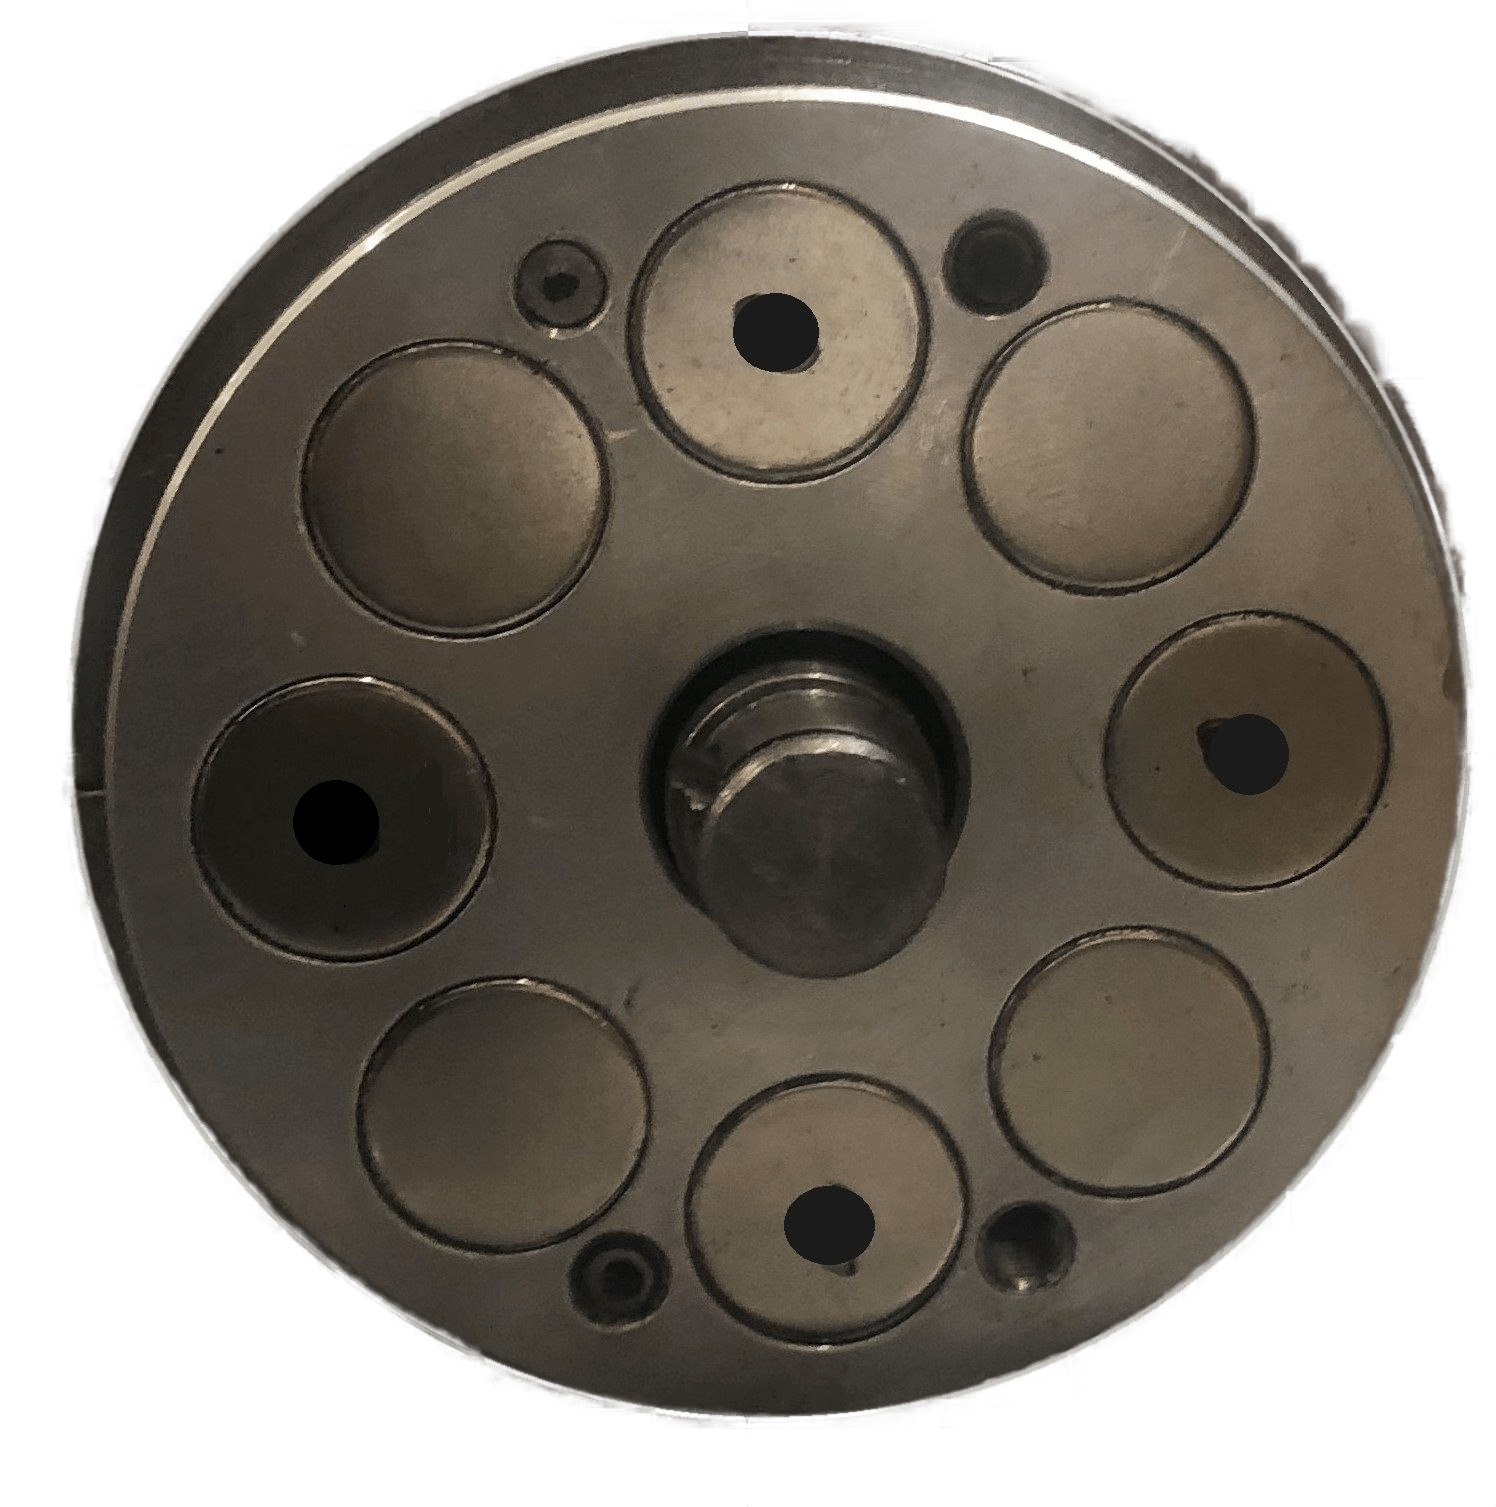
\includegraphics[height=0.8\linewidth]{BrakeArray.jpg}
		\caption{Built Magnet Array}
		\label{fig:magarr}
	\end{subfigure}%
	\hfill
	\begin{subfigure}{.4\textwidth}
		\centering
		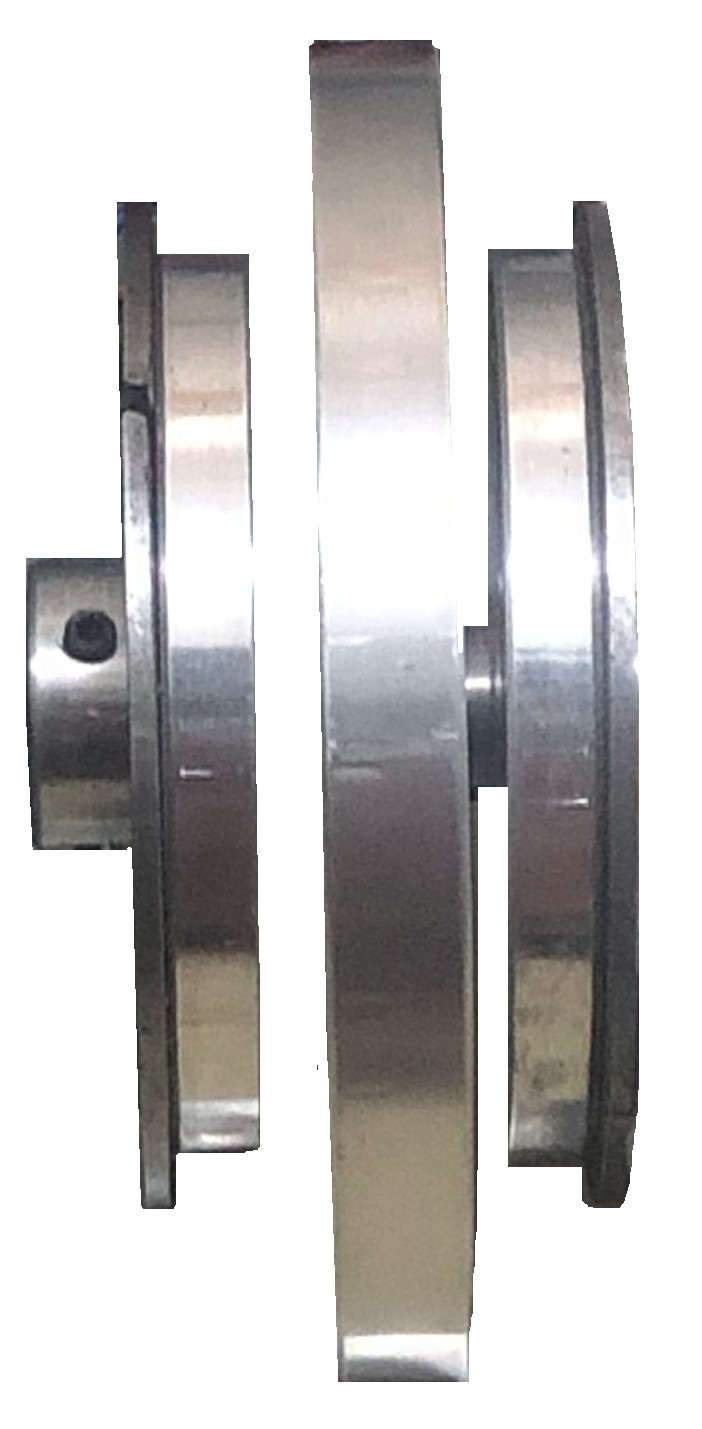
\includegraphics[height=0.8\linewidth]{BrakeView.jpg}
		\caption{Built Brake Configuration}
		\label{fig:brakefin}
	\end{subfigure}
	\caption{Built Eddy Current Brake}
	\label{fig:magets}
\end{figure}

\vspace*{-0.5cm}

Using Equation~\ref{eq:low}, Equation~\ref{eq:high} and Equation~\ref{eq:comb}, the theoretical torque curve shown in Figure~\ref{fig:BrakeDesign} is determined for the maximum braking condition. Figure~\ref{fig:BrakeDesign} also shows the braking power determined by Equation~\ref{eq:pow} for the designed brake parameters.

\begin{figure}[H]
	\centering
	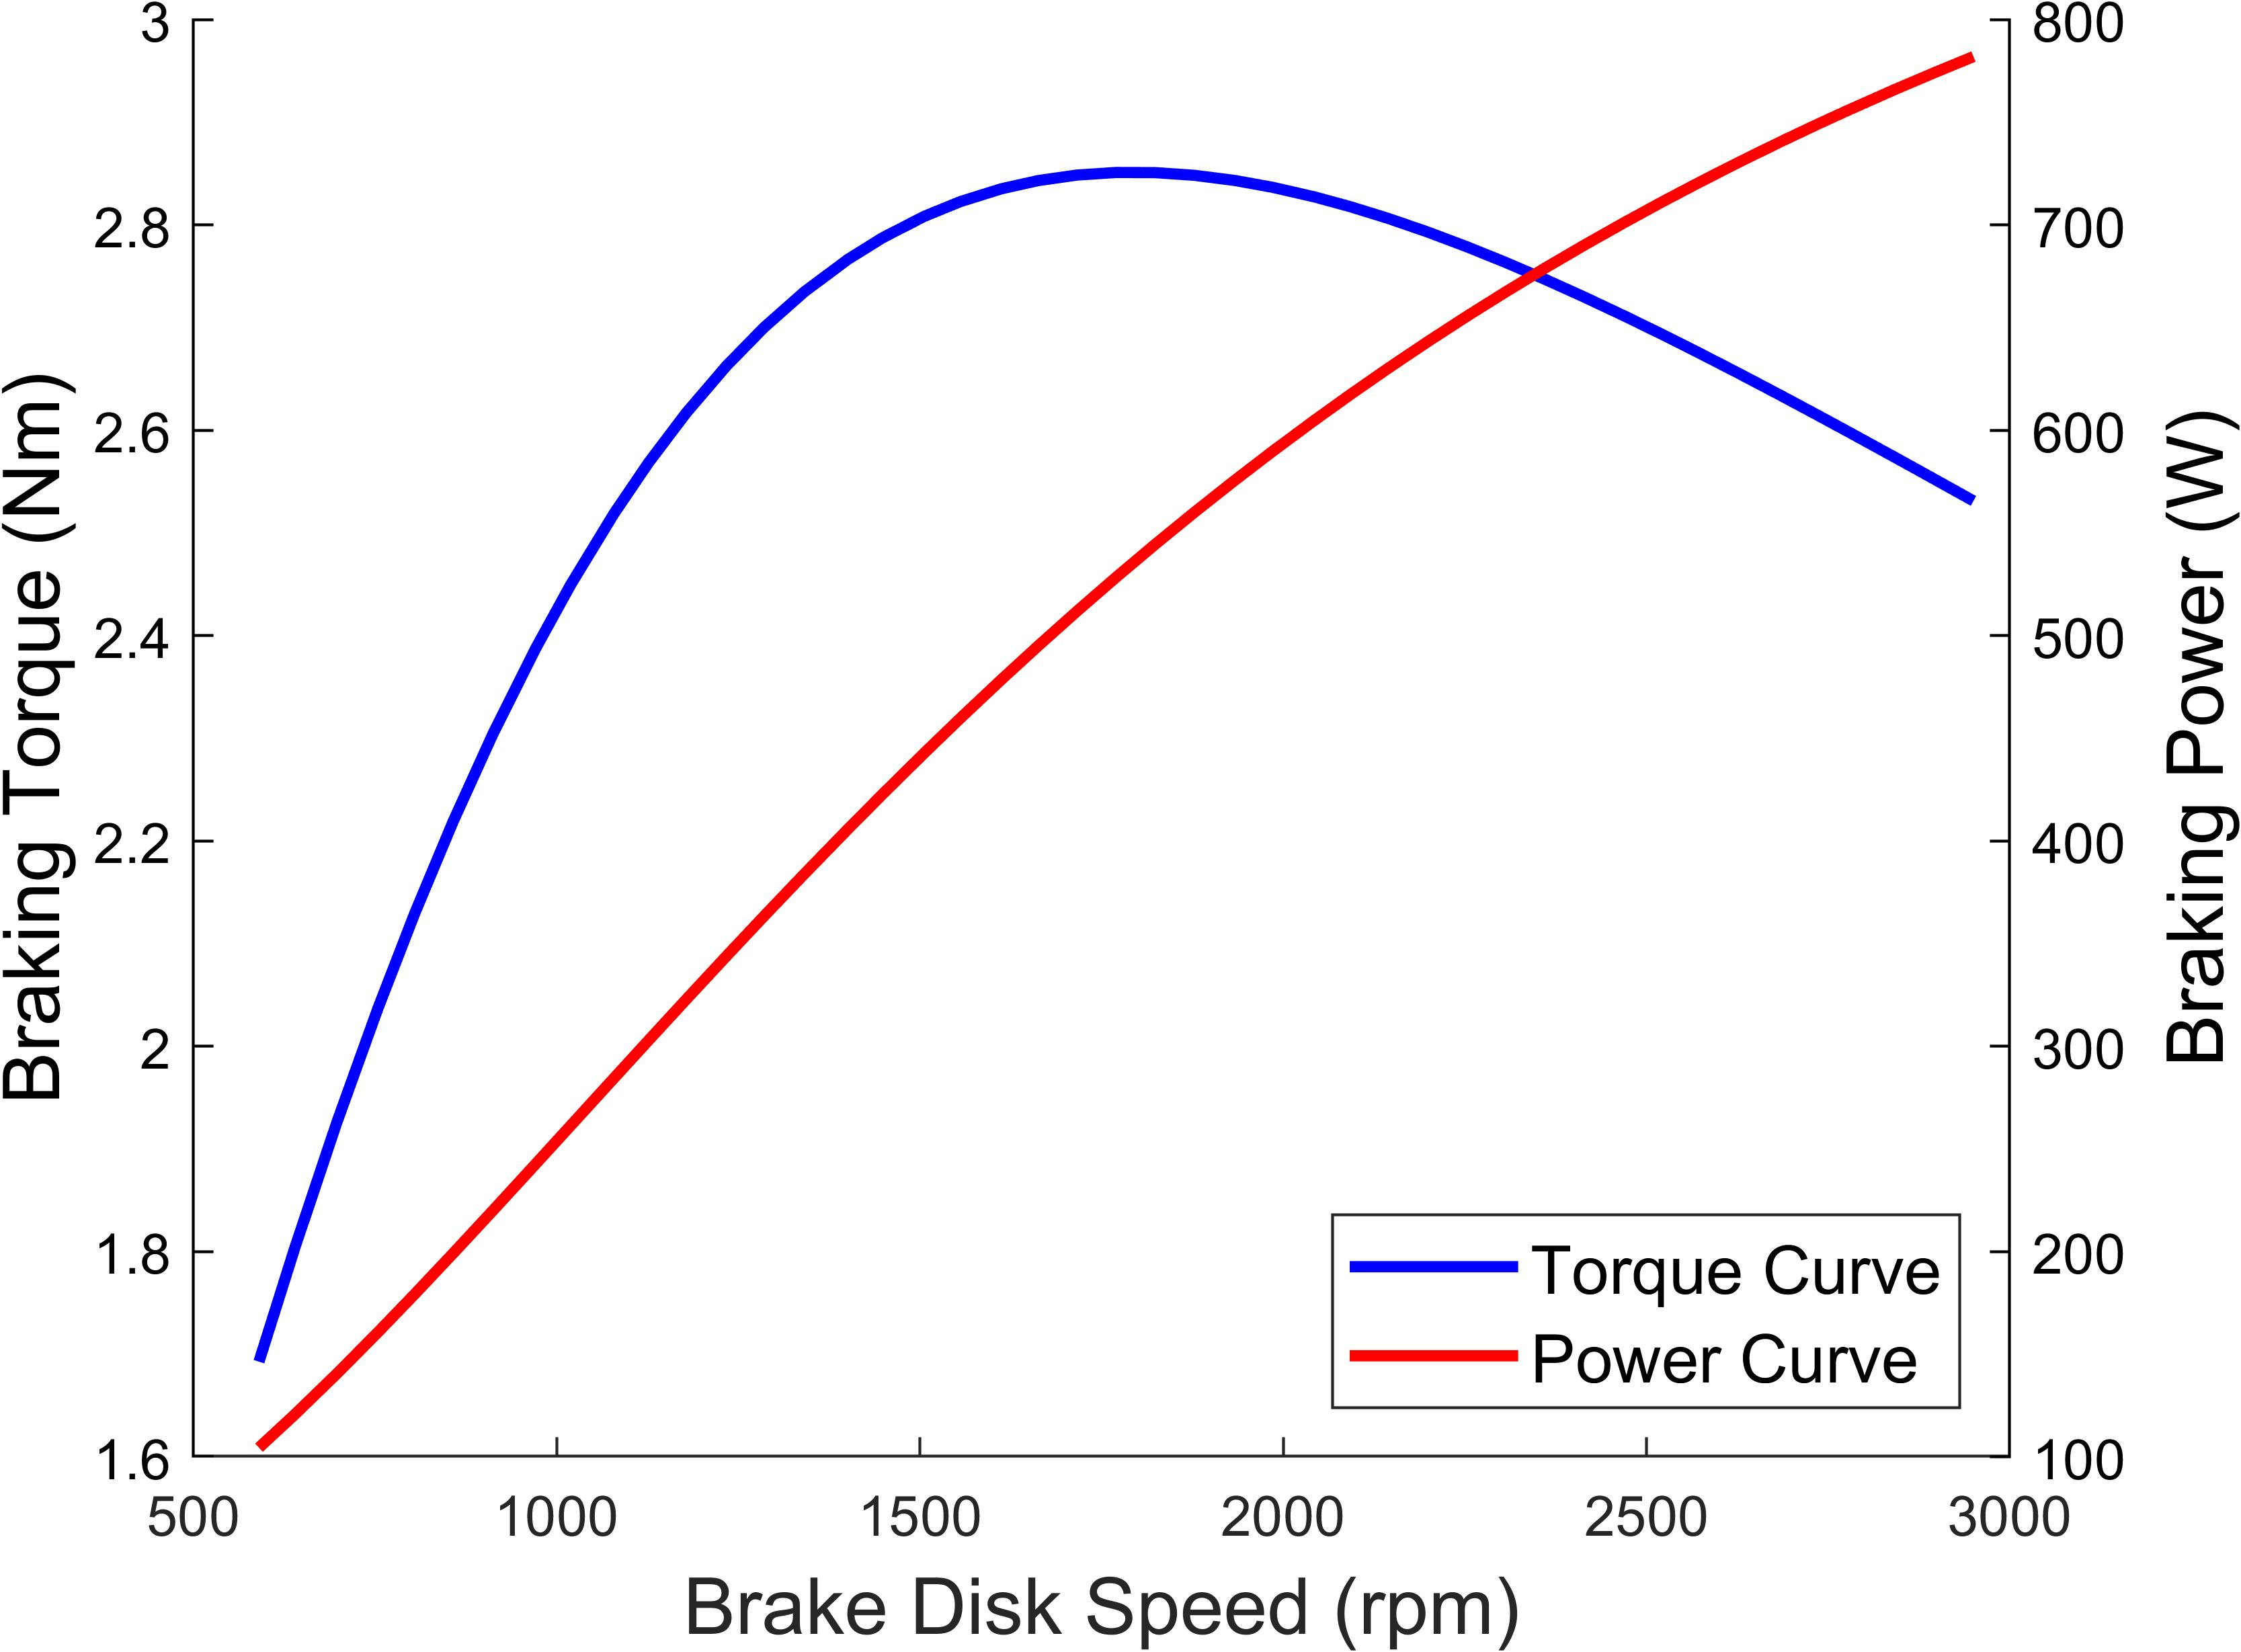
\includegraphics[width=0.6\textwidth]{BrakeDesign.jpg}
	\caption{Eddy Current Brake Design Results}
	\label{fig:BrakeDesign}
\end{figure}

\vspace*{-0.9cm}

\section{Frame Design}

The frame of the trainer consists of three separate sections. The rear section contains the power roller and one of the idle rollers. The front section contains the front idle roller and the middle section serves to connect the rear and front sections. Aluminium square tubes were used for the frame construction. Aluminium is an inexpensive and relatively light weight metal that is easy to manufacture.

\vspace*{-0.5cm}

\subsection{Rear Frame Section}

Figure~\ref{fig:RearDesign} is the designed rear section of the trainer. The eddy current brake is attached to the rear power roller and there is additional space next to the brake for mounting additional components and electronics. 

\begin{figure}[H]
	\centering
	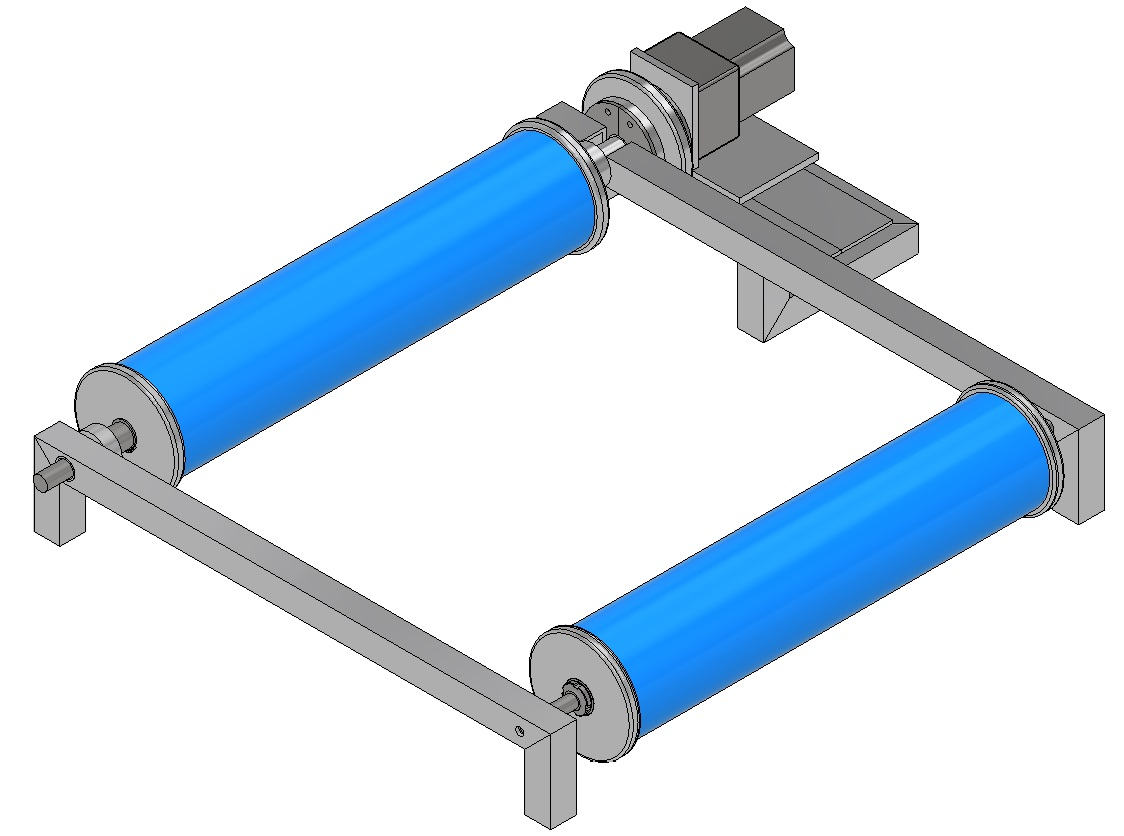
\includegraphics[width=0.4\textwidth]{RearFrameDesign.jpg}
	\caption{Rear Frame Section Design}
	\label{fig:RearDesign}
\end{figure}

\vspace*{-0.5cm}

The rollers are spaced much wider than on conventional roller trainers. This reduces the chance of the bicycle rolling forward off the trainer when braking torque is applied to the rear wheel.

Figure~\ref{fig:RearBuilt} shows the final assembly of the rear section of the frame with both the power roller and the idle roller attached. In Figure~\ref{fig:RearBuilt} the exposed end of the power shaft is clearly visible. This is where the test setup discussed in Chapter~\ref{ch:testing} attaches to the trainer.

\begin{figure}[H]
	\centering
	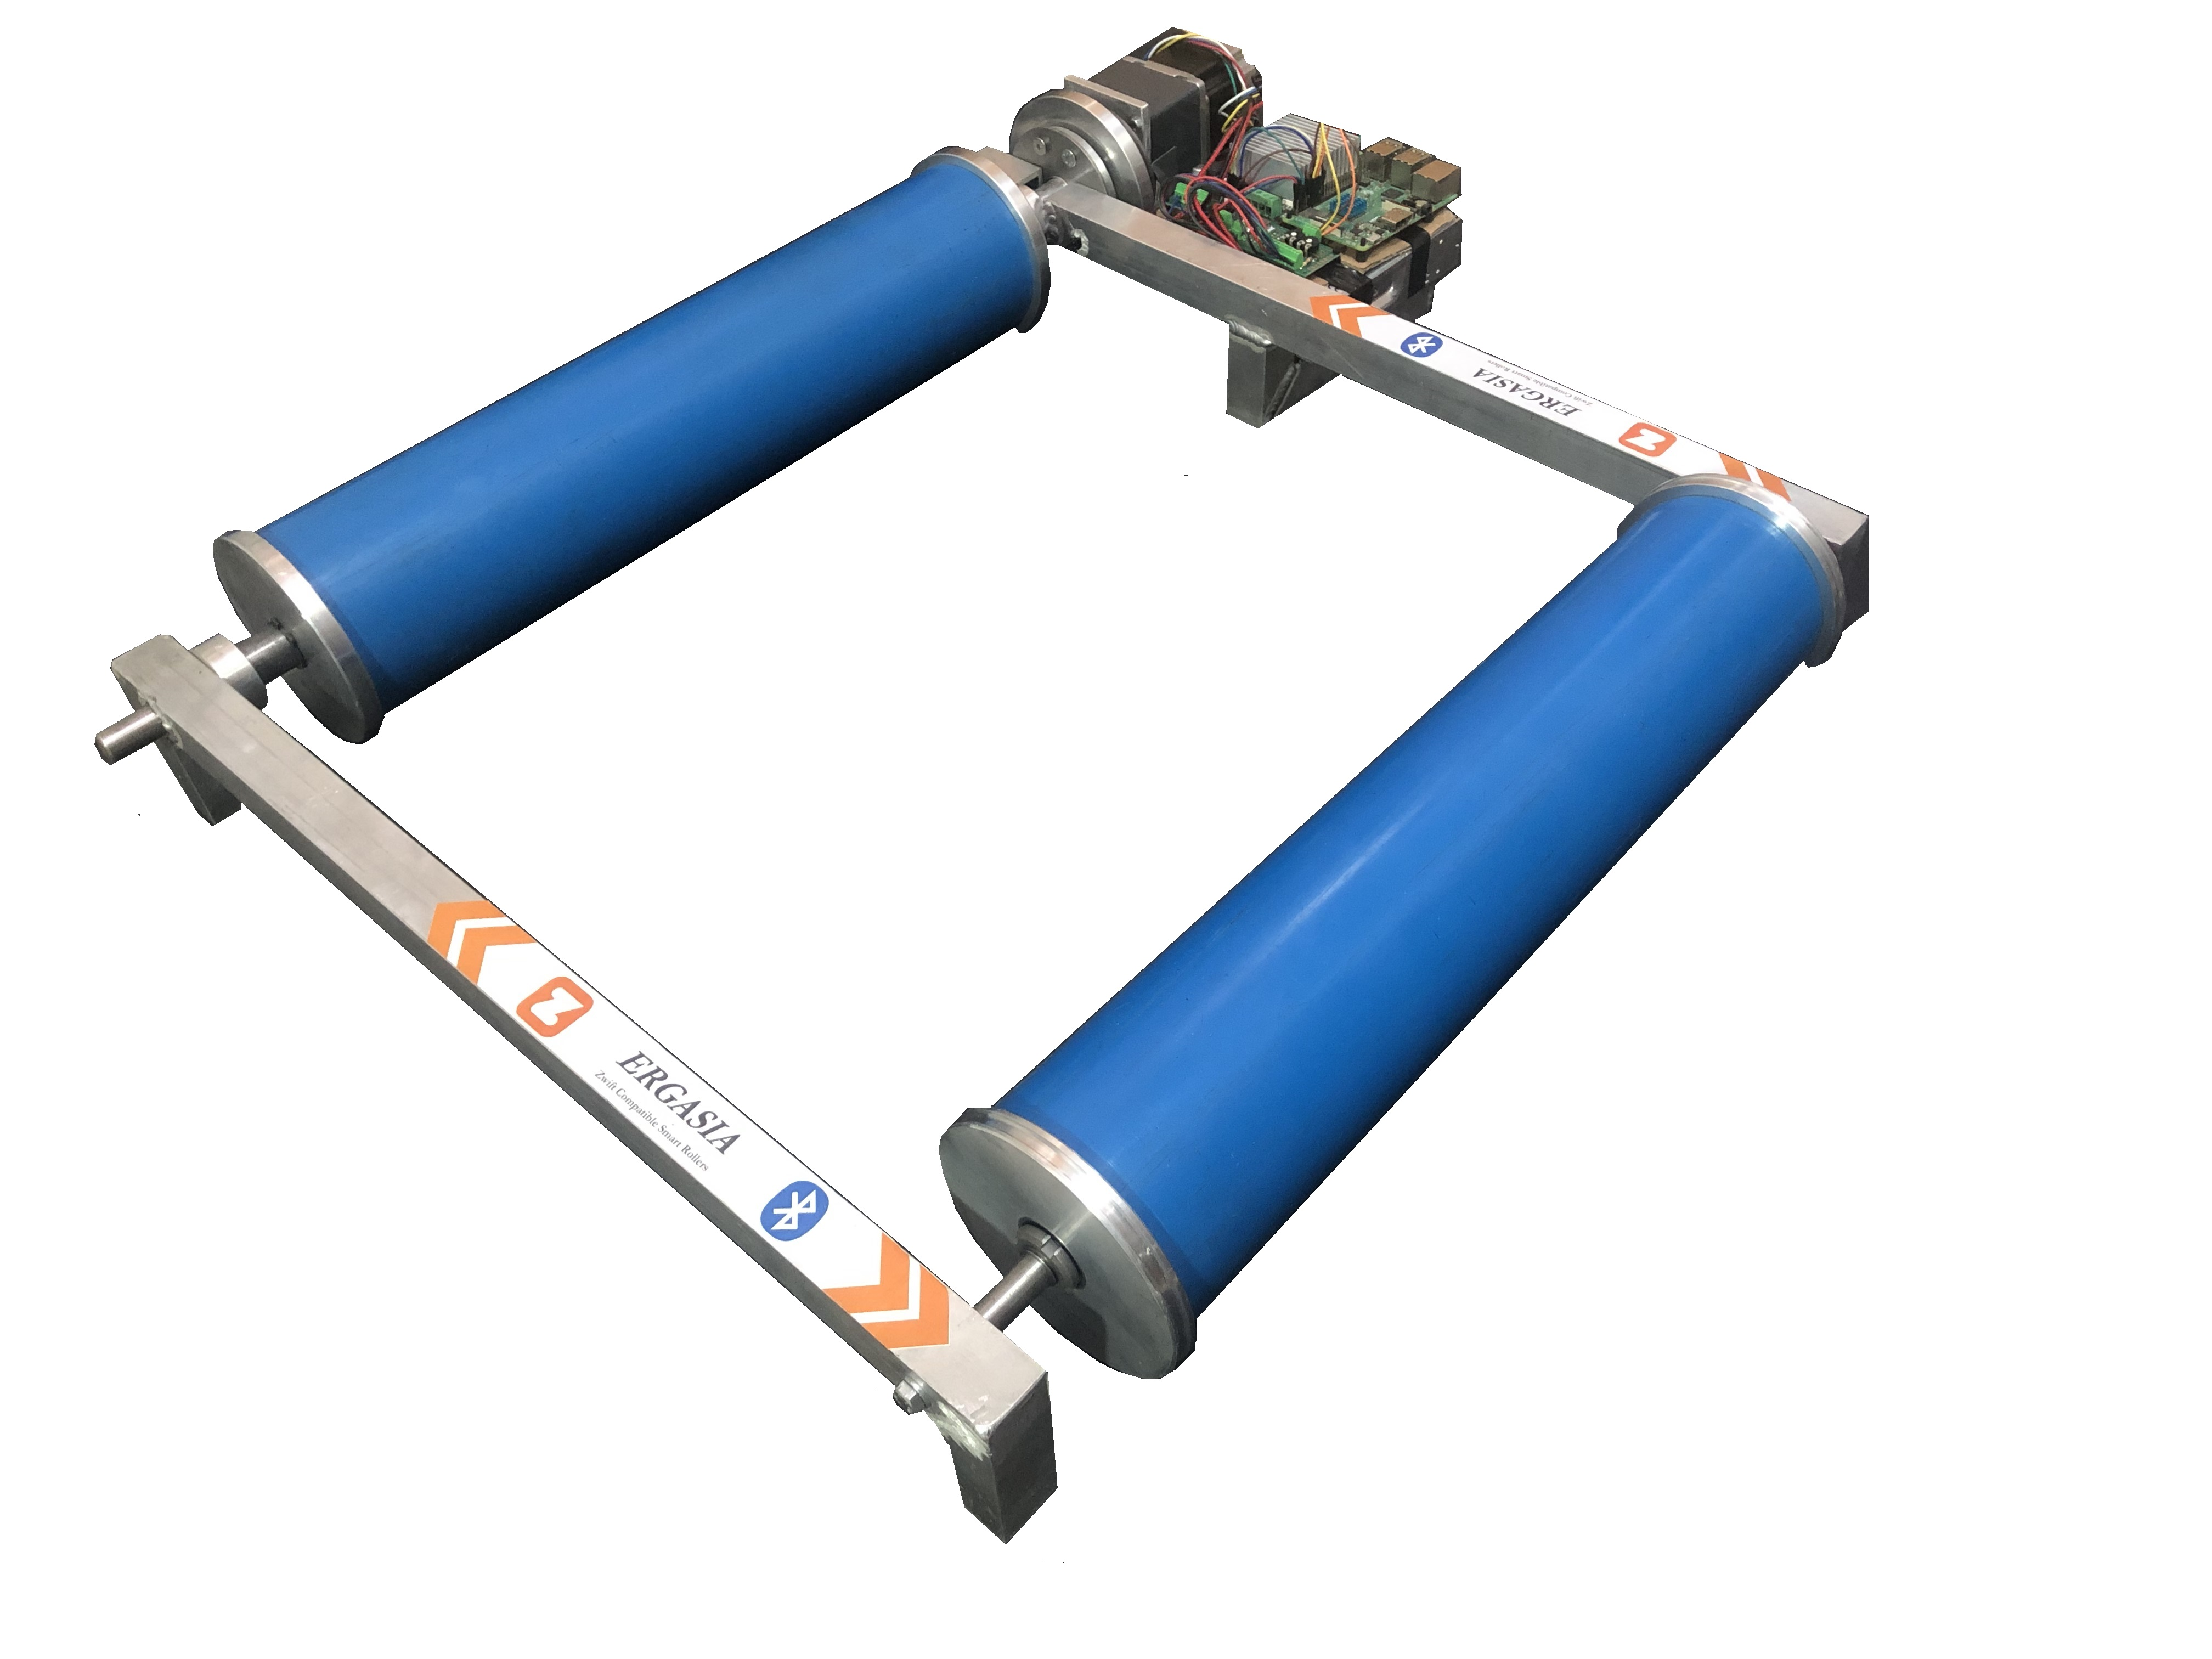
\includegraphics[width=0.5\textwidth]{RearFrameBuilt.jpg}
	\caption{Rear Frame Section Construction}
	\label{fig:RearBuilt}
\end{figure}

\vspace*{-0.8cm}

The speed of both rear rollers is being measured by optical tachometers. The idle roller rotating at a higher rate than the power roller indicates that the bicycle wheel is slipping on the power roller. This will cause additional wear on the bicycle tyre as well as the roller drum. Chapter~\ref{ch:software} demonstrates a solution to this by temporarily reducing the braking torque in order to allow the tyre to fully engage with the rear roller again. 

\vspace*{-0.3cm}

\subsection{Front Frame Section}

The front section of the frame is where the other idle roller is mounted. This is also where support for multiple wheelbase lengths was added, by providing multiple mounting options where the front idle roller can be attached to the frame pieces. The two sides of the front section are also connected by an aluminium rod that adds stability and rigidity to the trainer. Figure~\ref{fig:FrontDesign} shows the design that was created for the front section of the frame.

\begin{figure}[H]
	\centering
	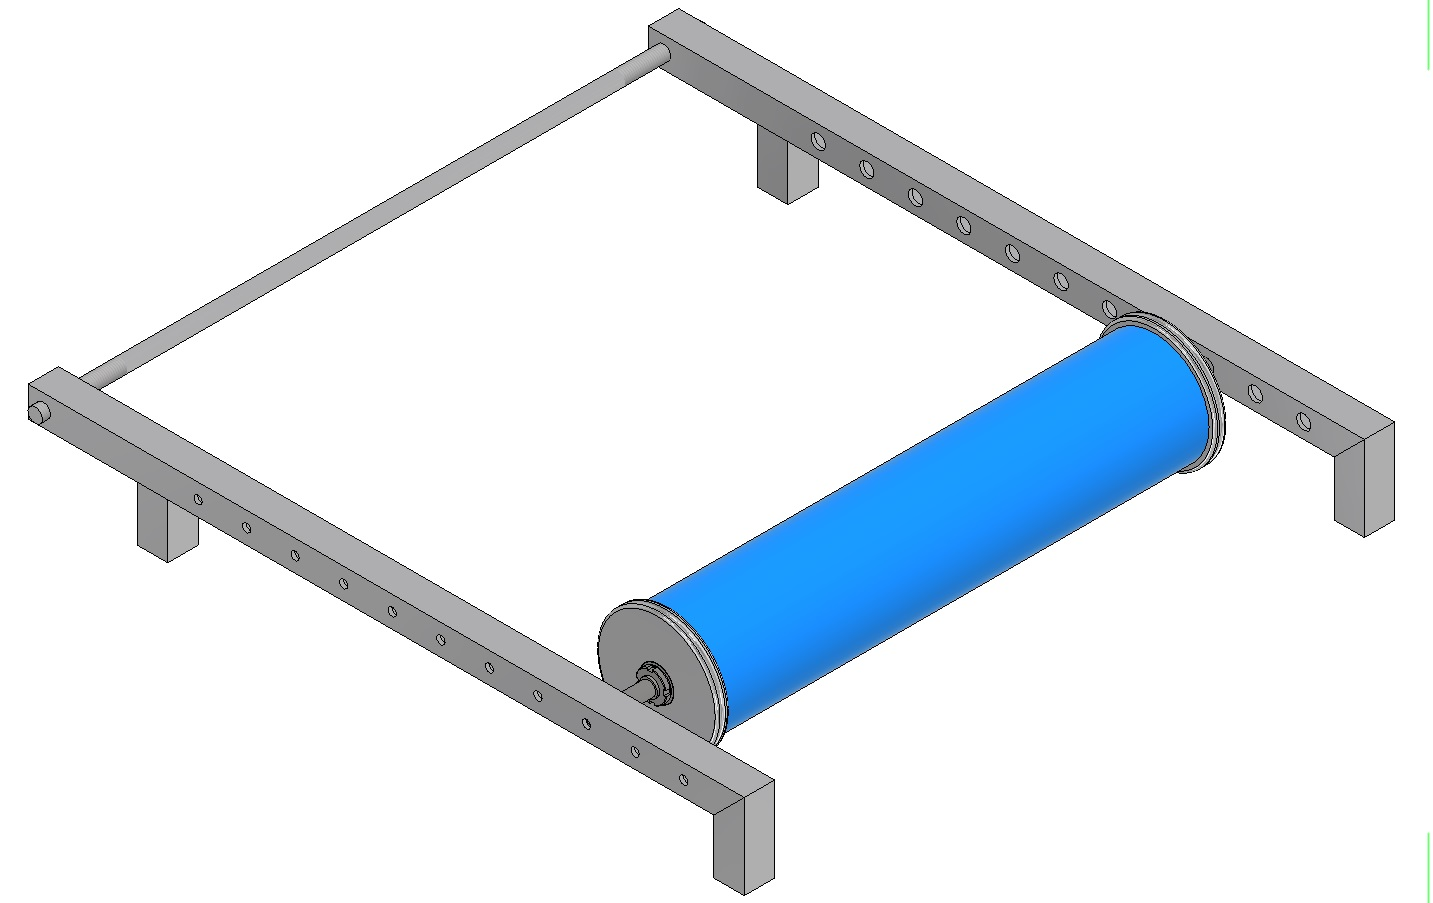
\includegraphics[width=0.4\textwidth]{FrontFrameDesign.jpg}
	\caption{Front Frame Section Design}
	\label{fig:FrontDesign}
\end{figure}

\vspace*{-0.5cm}

Figure~\ref{fig:FrontBuilt} shows the final constructed front section of the trainer with multiple mounting holes to allow for adjustment of the trainer length in order to accommodate a wider range of bicycle wheelbases. The front section is also lower to the ground than the rear frame section. This reduces the incline of the bicycle by about \SI{2}{\degree} and provides additional stability and familiarity to the cyclist.

\begin{figure}[H]
	\centering
	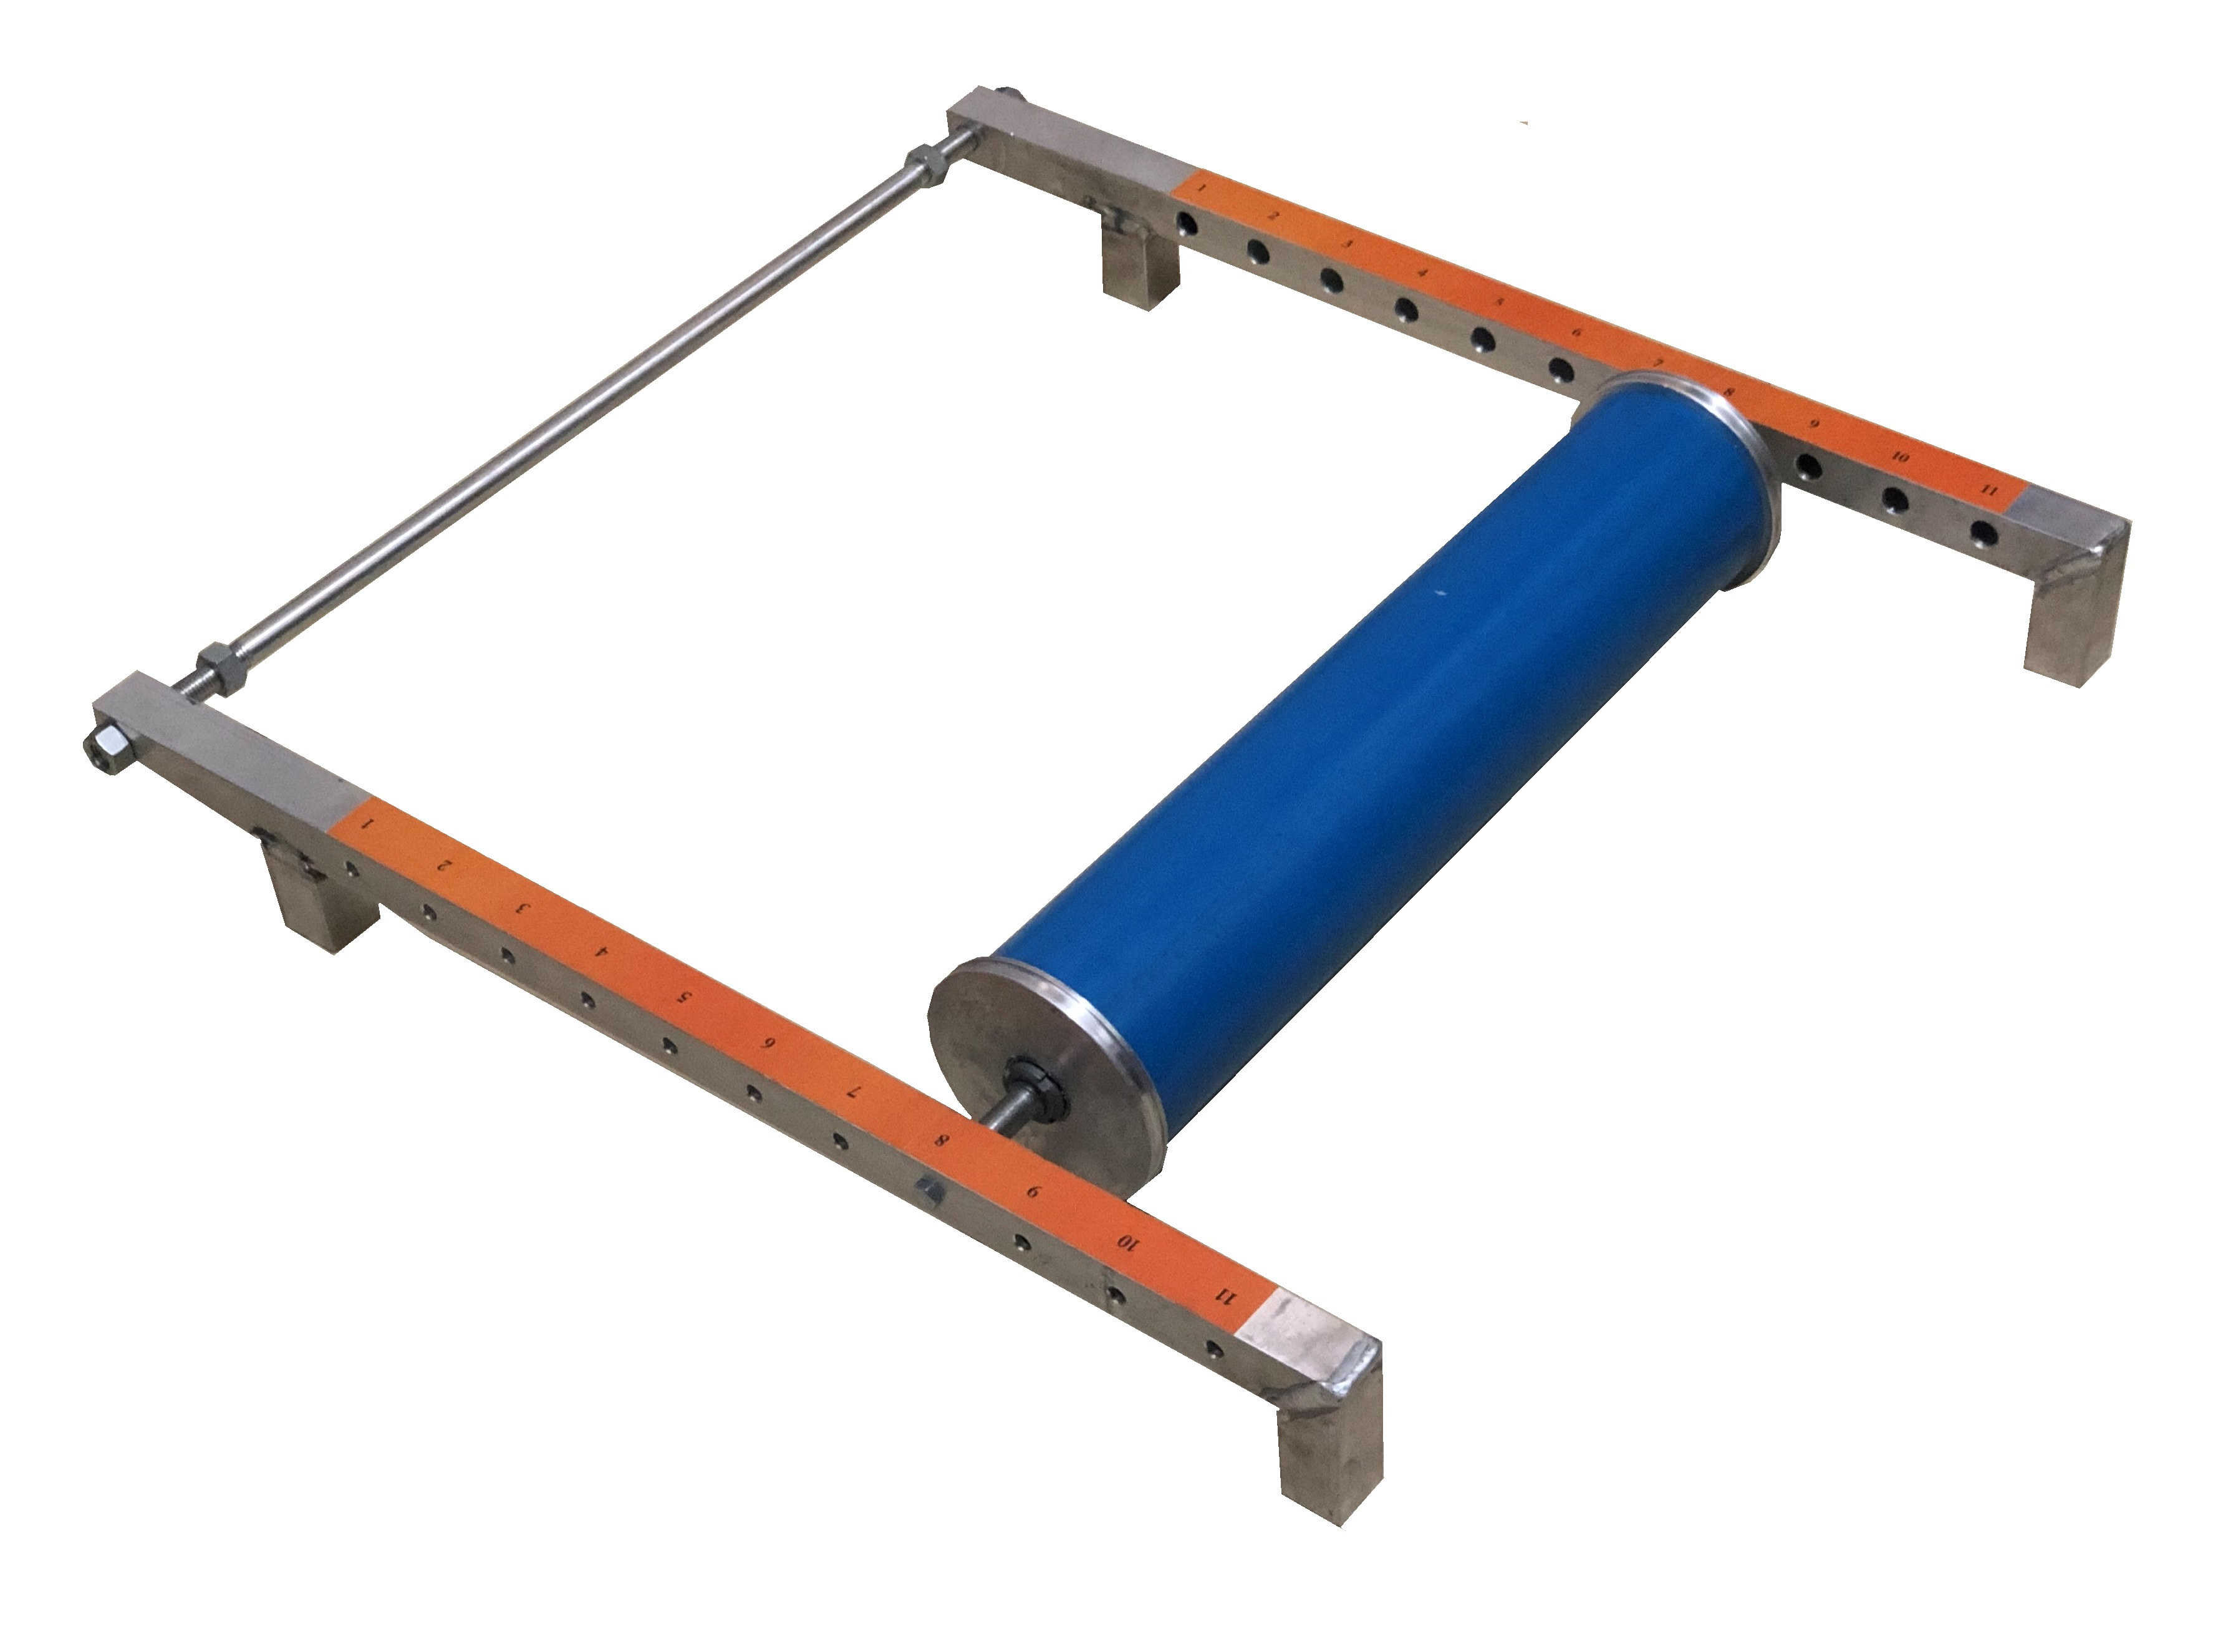
\includegraphics[width=0.6\textwidth]{FrontFrameBuilt.jpg}
	\caption{Front Frame Section Construction}
	\label{fig:FrontBuilt}
\end{figure}

\vspace*{-0.5cm}

Figure~\ref{fig:FrontBuilt} also shows the addition of numbered stickers that serve as a reference for positioning the roller on both sides of the frame. This also allows the user to easily configure the trainer for different bicycles after the correct length number has been found during the initial setup for that specific bicycle.

\section{Complete Frame}

Figure~\ref{fig:1} shows the final trainer that was designed and built in this project. The length is easy to adjust by moving the front idle roller to different mounting positions.

\begin{figure}[H]
	\centering
	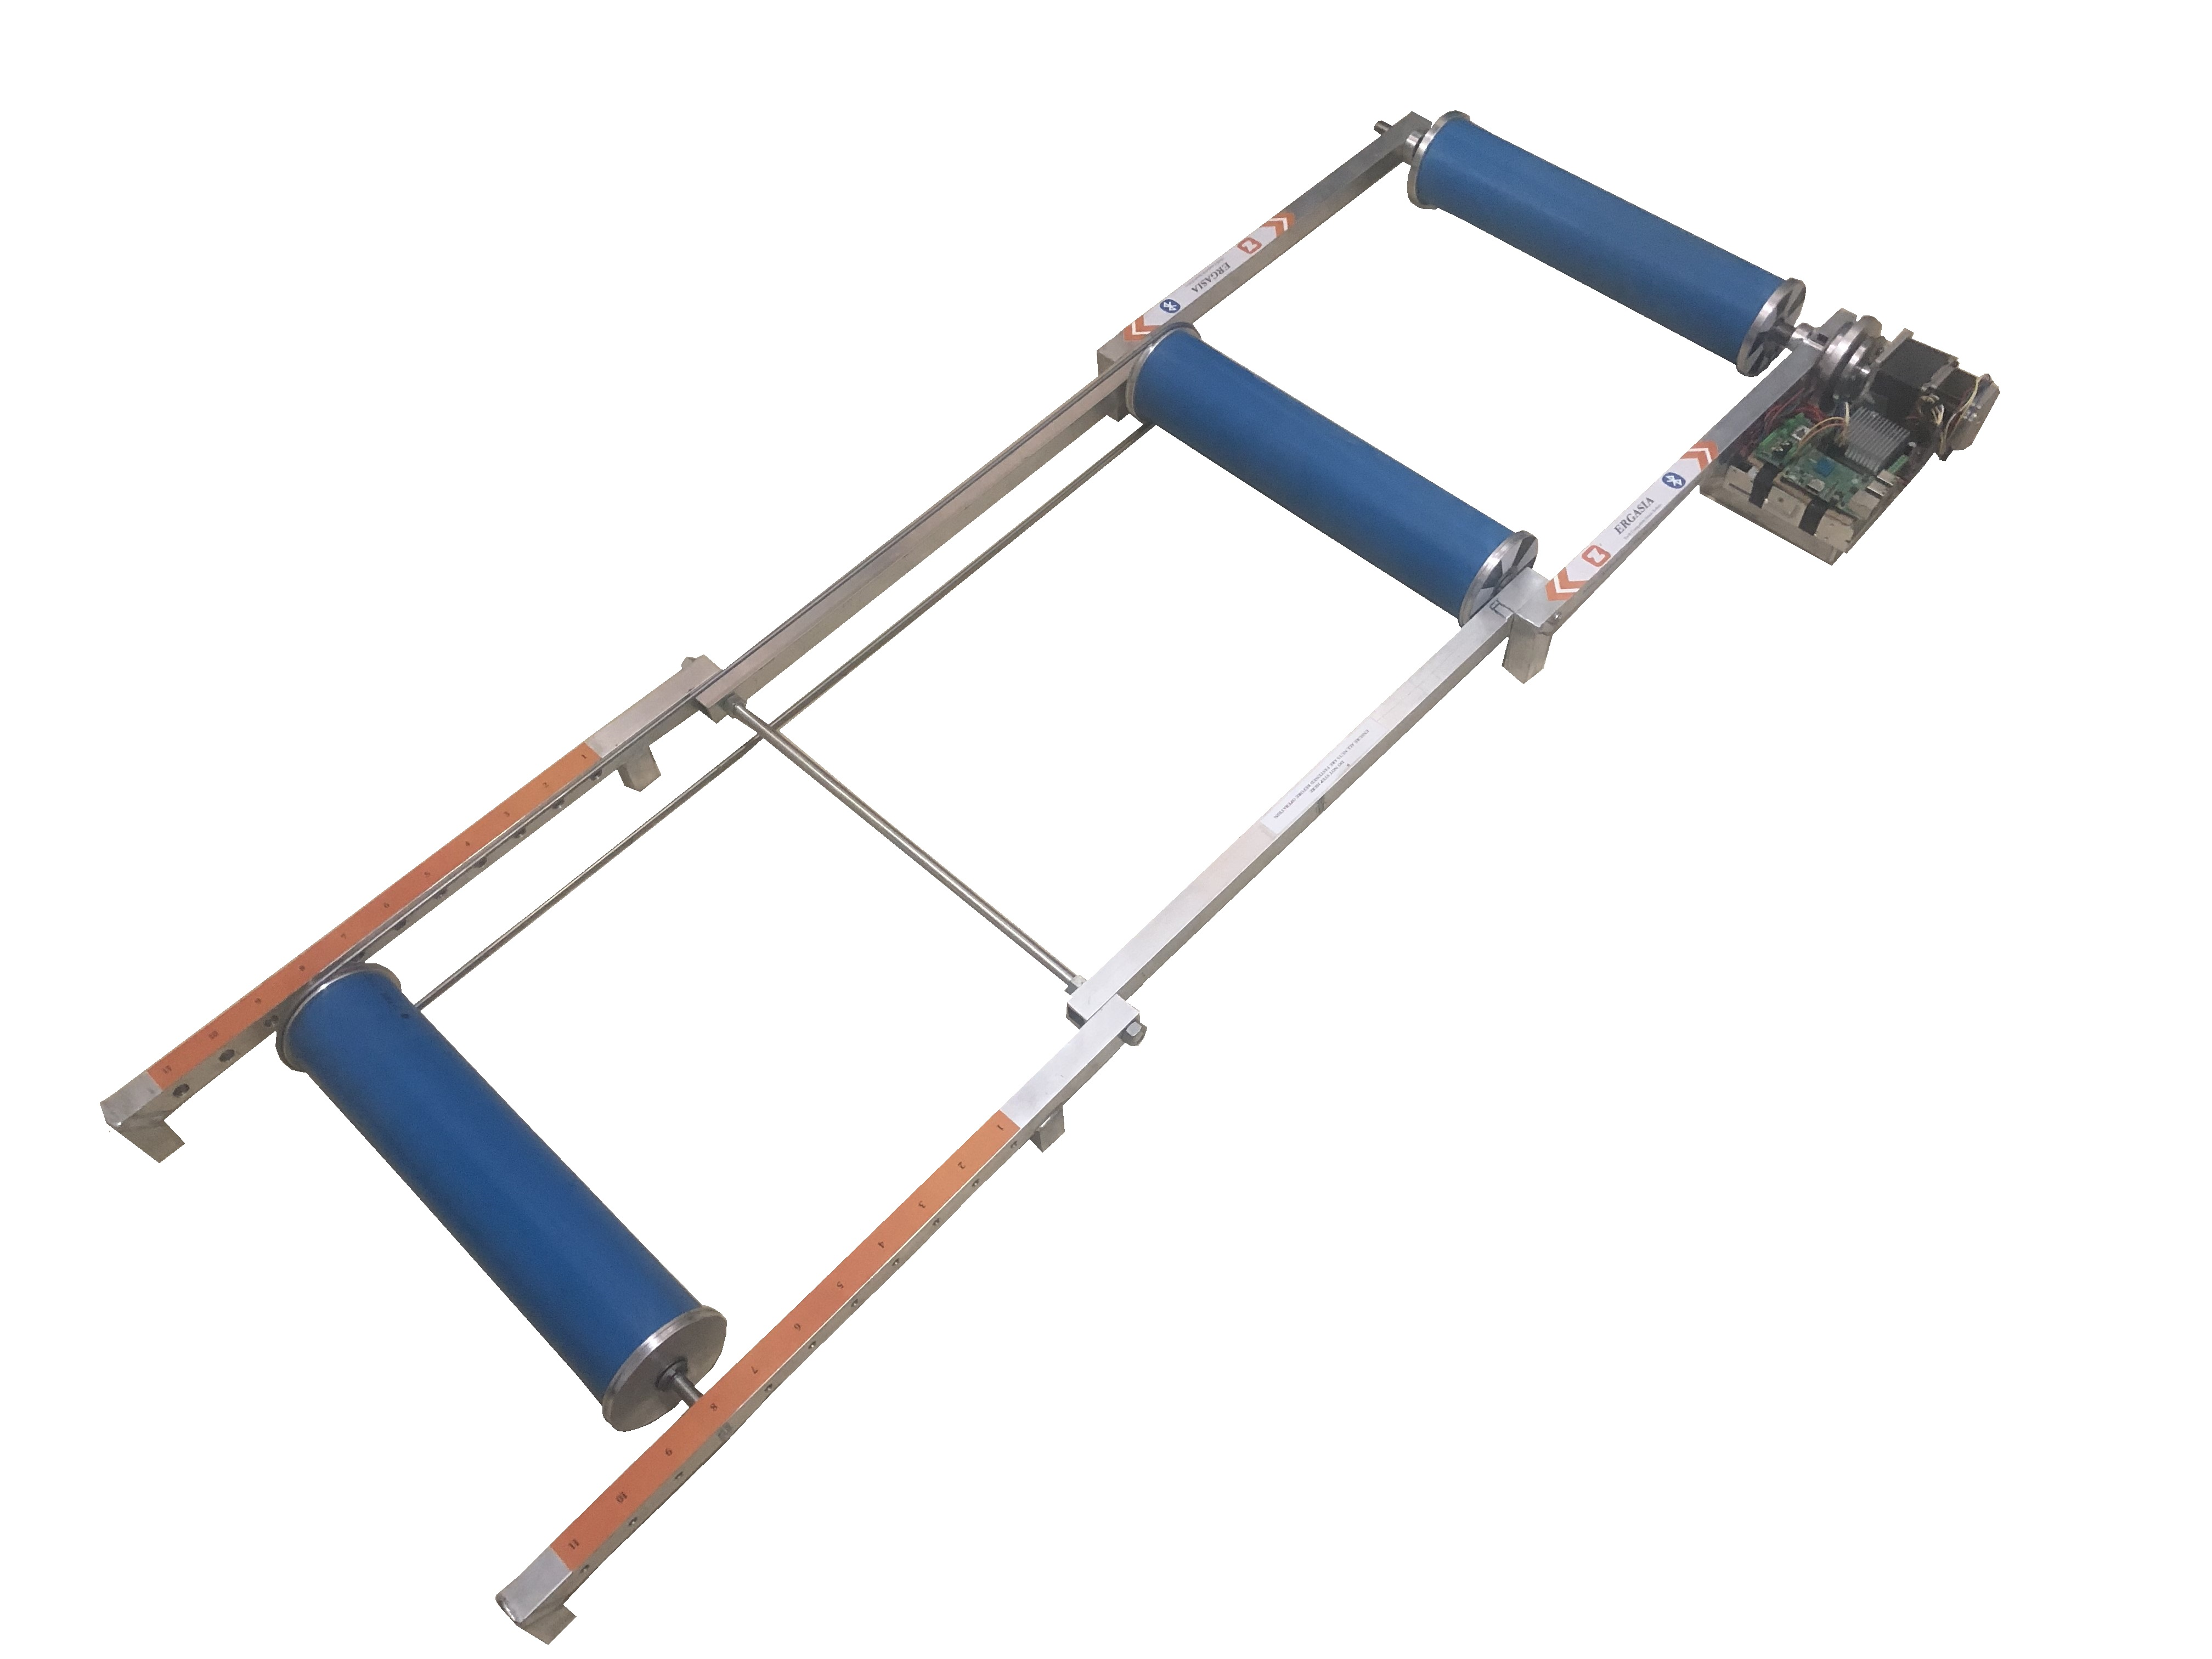
\includegraphics[width=0.6\textwidth]{FrameFull.jpg}
	\caption{Final Assembled Trainer}
	\label{fig:1}
\end{figure}

\vspace*{-0.5cm}

Figure~\ref{fig:2} shows the final model folded into the compact storage configuration. This allows for easy transport and storage of the trainer while also protecting the speed sensors when the trainer is not in use.

\begin{figure}[H]
	\centering
	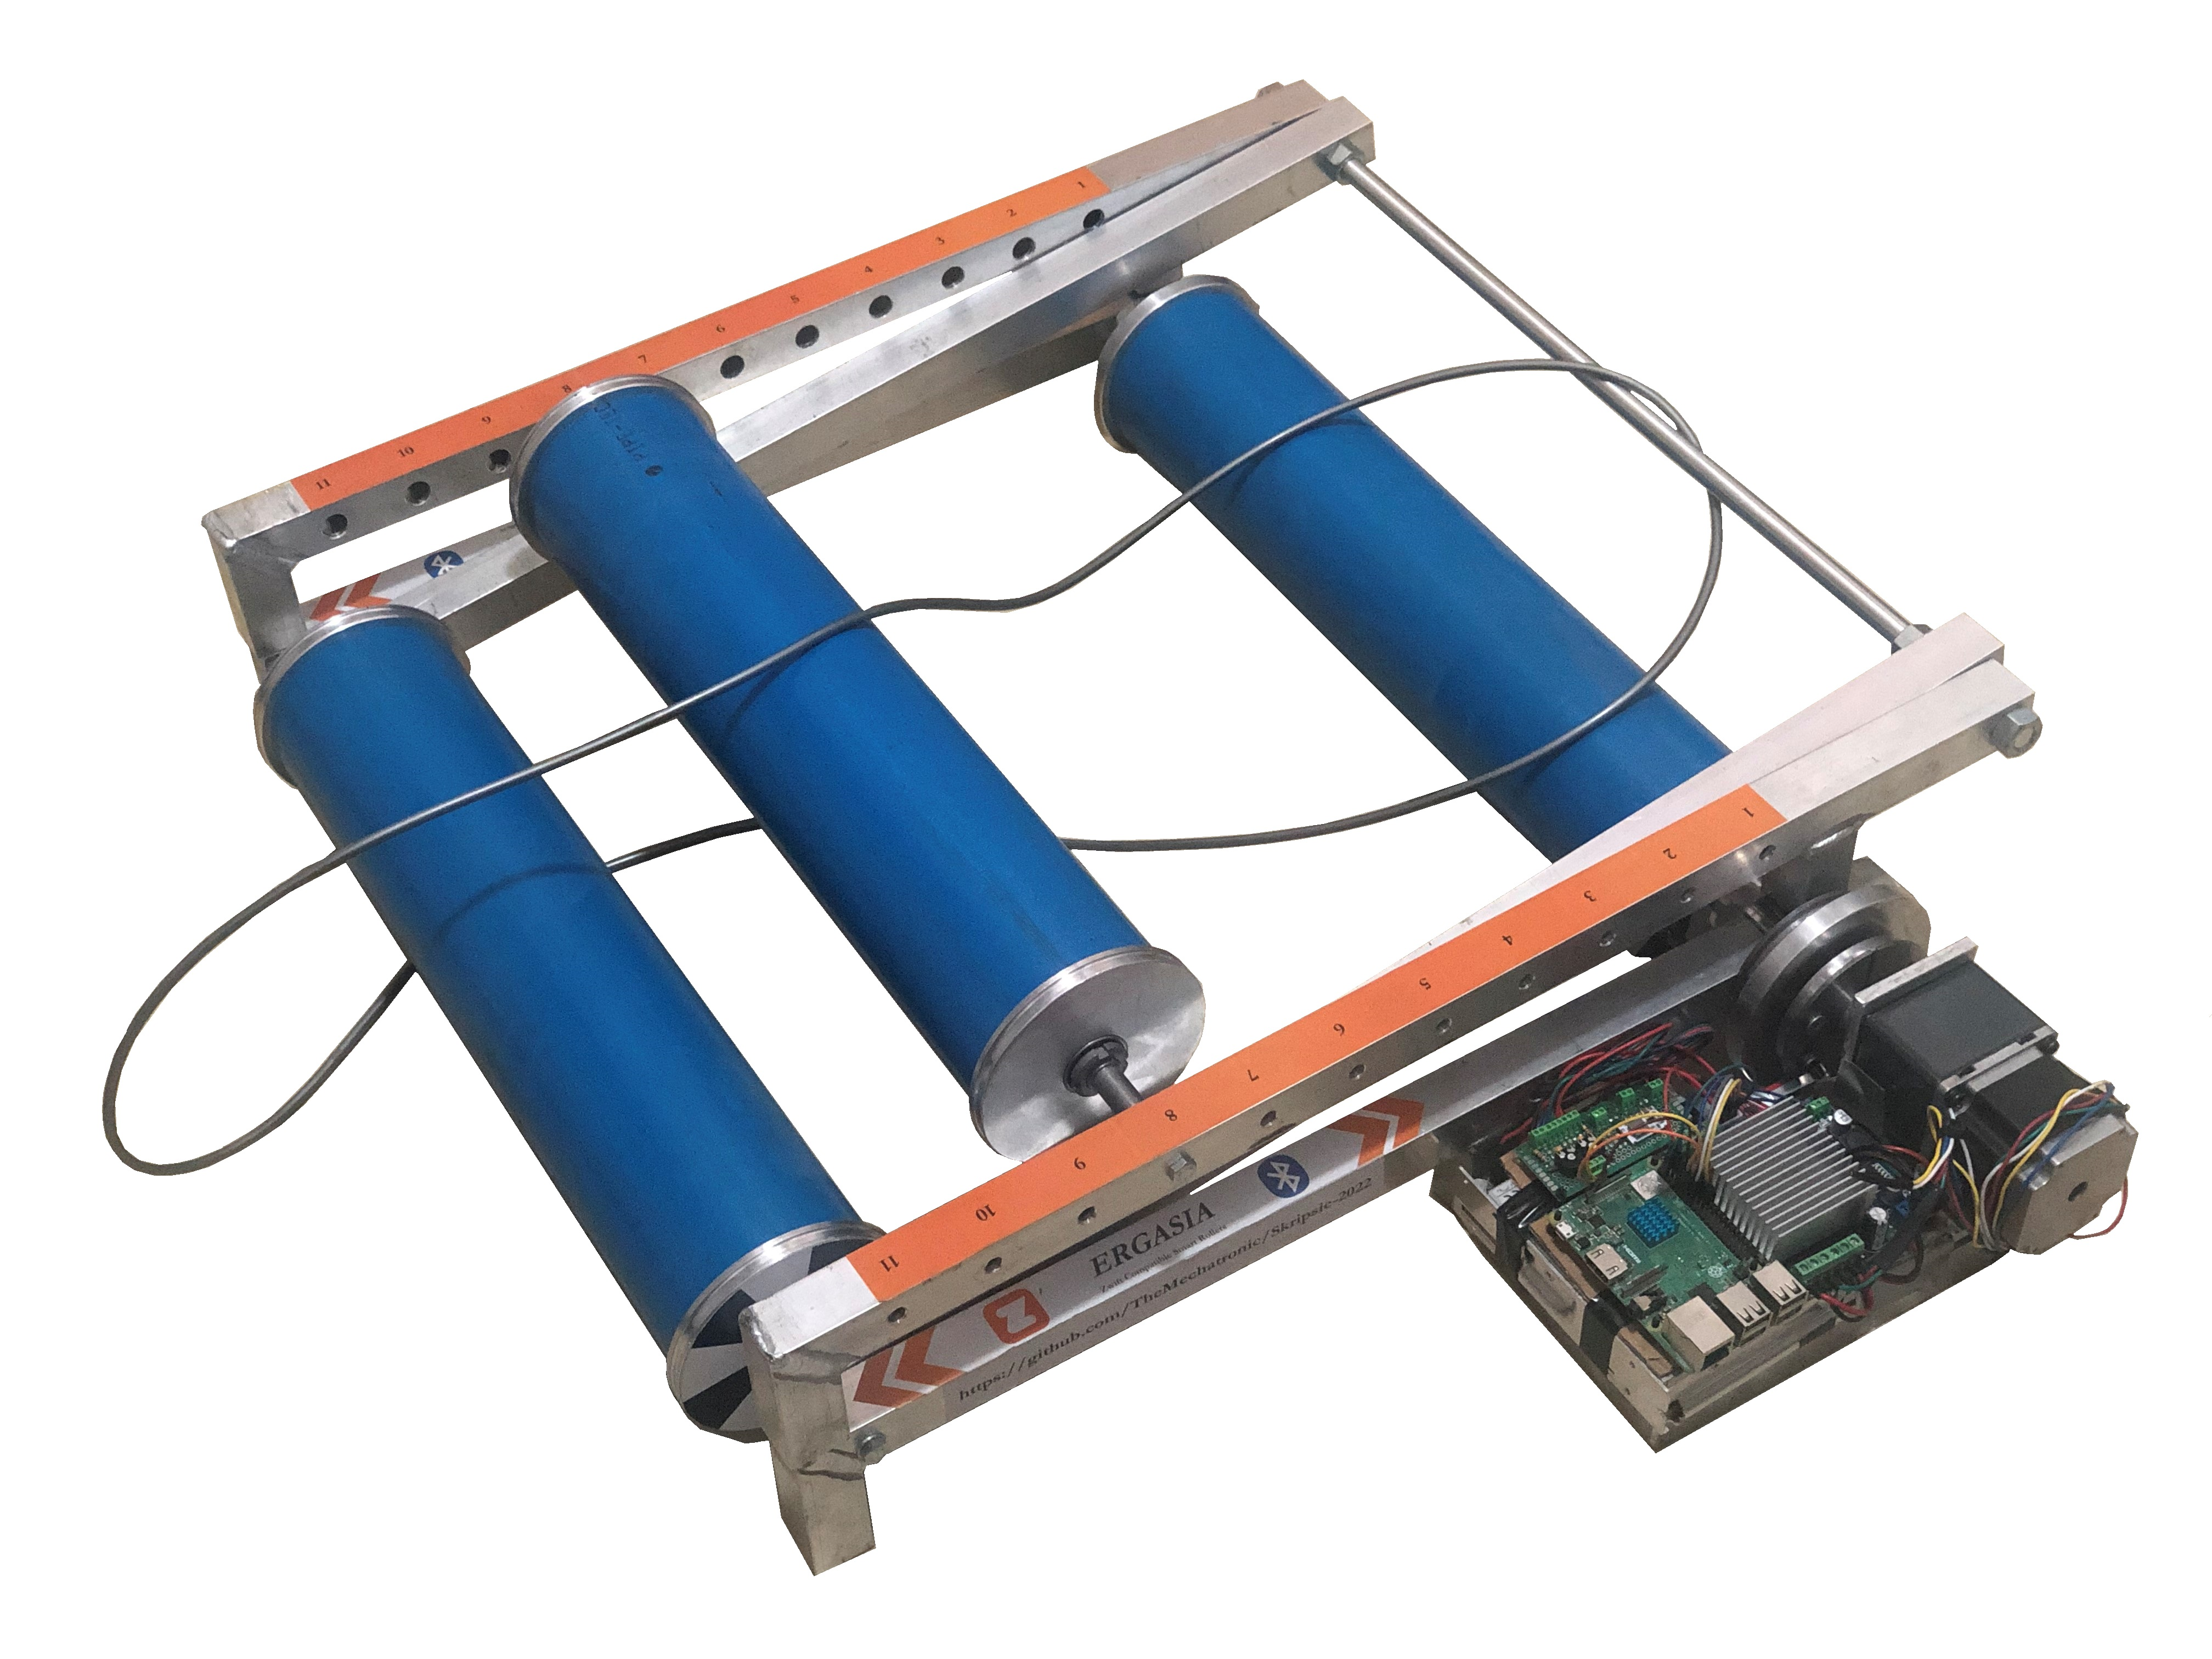
\includegraphics[width=0.5\textwidth]{FrameFold.jpg}
	\caption{Compact Folded Trainer Assembly}
	\label{fig:2}
\end{figure}

\vspace*{-0.5cm}

The aluminium frame and rollers prove to be very stable even while supporting the weight of a cyclist with a bicycle.